\documentclass[a4paper,11pt]{article}
\pdfoutput=1

\usepackage[UKenglish]{babel}
\usepackage{csquotes}
\usepackage{jheppub}
\usepackage[T1]{fontenc}
\usepackage{listings}
\usepackage{lmodern}
\usepackage[binary-units=true]{siunitx}
\usepackage{xcolor}

\newcommand{\alphas}{\alpha_\mathrm{s}}

\title{Including EW and mixed QCD-EW corrections into PDF fits}

\author[a]{S. Carrazza,}
\author[b]{E. Nocera,}
\author[a]{C. Schwan}
\author[a,b]{and M. Zaro}

\affiliation[a]{Tif Lab, Dipartimento di Fisica, 
Universit\`a di Milano and INFN, Sezione di Milano, 20133 Milano, Italy}
\affiliation[b]{Nikhef Theory Group, Science Park 105, 1098 XG Amsterdam, 
The Netherlands}

\emailAdd{stefano.carrazza@mi.infn.it}
\emailAdd{e.nocera@nikhef.nl}
\emailAdd{christopher.schwan@mi.infn.it}
\emailAdd{marco.zaro@mi.infn.it}

\abstract{}

\begin{document}

\maketitle
\flushbottom

\section{Introduction}
\label{sec:introduction}

With the recent completion of Run II, the Large Hadron Collider (LHC) has 
accumulated data from an integrated luminosity of approximately 
\SI{150}{\per\femto\barn}~\cite{Mangano:2020icy}. This represents only a small fraction of
the anticipated \SI{3000}{\per\femto\barn} that will eventually be recorded in the
forthcoming twenty years of LHC operation. Nevertheless the statistical 
uncertainty of the data has already shrunk to unprecedentedly small values,
typically \SI{1}{\percent} or less, a fact that will allow for precision tests of the
Standard Model (SM) and for indirect searches of New Physics only if 
theoretical predictions become comparatively precise. This entails the 
computation of additional higher-order contributions to the fixed-order 
perturbative expansion, on the one hand, and an increasingly
sophisticated determination of the Parton Distribution Functions (PDFs) of the 
proton~\cite{Gao:2017yyd,Ethier:2020way}, on the other hand. 

In the first respect, because Quantum Chromodynamics (QCD) dominates the 
interactions occurring within colliding protons at the LHC, much effort 
has been devoted to the computation of higher-order QCD corrections: 
fully-differential next-to-leading order (NLO) results, possibly matched to a
parton shower, are currently automated in various general-purpose
Monte Carlo generators~\cite{Gleisberg:2008ta,Alwall:2014hca,Bellm:2015jjp}
(see also ref.~\cite{Buckley:2011ms} for a review),
while an increasing number of next-to-next-to-leading order (NNLO) predictions 
are becoming available for processes with various degrees of inclusiveness
(see e.g.\ ref.~\cite{Amoroso:2020lgh} and references therein). The computation
of higher-order corrections in the electroweak (EW) and combined QCD+EW theory has
also witnessed a comprehensive progress. Frameworks 
were developed in which the QCD and EW couplings are simultaneously treated as 
small parameters in the perturbative expansion, and the computation of 
theoretical predictions, accurate to NLO in both (including multi-coupling
QCD--EW terms), is automated~\cite{Kallweit:2014xda,Biedermann:2017yoi,Frederix:2018nkq}. For an extensive and recent review, see ref.~\cite{Denner:2019vbn}.

In the second respect, contemporary PDF
sets~\cite{Harland-Lang:2014zoa,Ball:2017nwa,Hou:2019efy}
incorporate a significant amount of LHC data, which is analysed with NNLO QCD 
theory by default. No EW corrections are systematically included in the 
theoretical description of the experimental observables to which PDFs are 
optimised, except for QED effects if a photon PDF is 
determined~\cite{Martin:2004dh,Ball:2013hta,Schmidt:2015zda,Manohar:2016nzj,Manohar:2017eqh,Bertone:2017bme,Harland-Lang:2019pla}. The QED contribution is
included in the matrix element (at the lowest order for the LHC
processes considered) and in the DGLAP splitting
functions at leading order~\cite{Bertone:2013vaa}. Inclusion of NLO QCD--QED
combined corrections in the evolution is in principle also
possible~\cite{deFlorian:2015ujt}, and should be required to analyse the data
within consistent perturbative accuracy if higher-order EW and QCD corrections
are also included in partonic cross sections.
The resulting relative PDF uncertainty --- which accounts only for the
uncertainty of the data and of residual methodological inefficiencies inherent to 
each PDF determination --- can be as low as \SI{1}{\percent} at the EW
scale~\cite{Ball:2017nwa}. Theoretical uncertainties, possibly of comparable 
size (e.g.\ from missing higher-order terms in the QCD perturbative
expansion), have started to be represented 
into PDF uncertainties only very 
recently~\cite{AbdulKhalek:2019bux,AbdulKhalek:2019ihb}.

The two respects are intertwined, as they both concur to determine the accuracy
of the theoretical predictions that are matched to the precision of the data.
In particular, taking advantage of the automation pioneered
in refs.~\cite{Kallweit:2014xda,Biedermann:2017yoi,Frederix:2018nkq},
perturbative corrections that arise from the simultaneous expansion in both the
QCD and EW couplings should start to be
incorporated in calculations for LHC processes as standard. The reason is
twofold. First, one expects NNLO QCD and NLO EW corrections to be of
comparable size because, at the EW scale, the QCD and EW running couplings 
become similar, $\alphas^2\sim \alpha$. If NNLO QCD corrections are included
by default in the computations, NLO EW corrections should be
taken into account as well. Second, the virtual exchange of soft or 
collinear weak bosons leads to Sudakov 
logarithms~\cite{Denner:2000jv,Denner:2001gw}
(see also ref.~\cite{Denner:2019vbn} and references therein),
which can make the coefficients of the EW series grow faster than 
their QCD counterparts. This behaviour is relevant in
phase-space regions associated with large mass scales (roughly of the order
of a \si{\tera\electronvolt}), where several LHC data sets (e.g.\ Z-boson
transverse-momentum distributions) enter both the validation of the SM and the search
for new physics.

The consistent inclusion of QCD and EW corrections in precision computations for
LHC processes entails
the solution of two separate problems. First, a problem of efficiency:
fast-interpolation grids should be constructed, whereby partonic matrix 
elements, accurate to NLO QCD+EW, are precomputed in such a way that the 
numerical convolution with generic input PDFs can be efficiently approximated
by means of interpolation techniques. Such grids are essential
whenever the evaluation of the hadronic cross section needs to 
be performed a large number of times, as is the case in the evaluation of
scale variations or of PDF fits. While two formats already exist for
these grids, \textsc{APPLgrid}~\cite{Carli:2010rw} and
\textsc{fastNLO}~\cite{Kluge:2006xs,Wobisch:2011ij,Britzger:2012bs}, none of them supports the inclusion of EW
corrections nor the interface to a Monte Carlo generator accurate to 
NLO QCD+EW\@. Second, a problem of consistency: the way in which EW effects may
(or may not) be folded into the data varies across different experimental 
analyses, a fact that challenges their consistent theoretical interpretation. 
Examples are the subtraction of background processes which should not be 
considered as such (e.g.\ the $t$-channel photon-induced component in
neutral-current Drell--Yan, which is not a separate process beyond leading
order) or of just a part of the EW effects (e.g.\ multiple-photon
radiation from light particles in the final state of neutral- or charged-current
Drell--Yan, especially with electrons). Be that as it may, if EW effects are
systematically included in theoretical predictions, they should not be subtracted
from experimental results, otherwise they will be double counted.

In this paper we address the first of these two problems. Specifically, 
we develop \textsc{PineAPPL}, a library that allows any user to generate
fast-interpolation grids, accurate to any fixed order in the QCD and
EW couplings. The library supports variations of the factorisation
and renormalisation scales, and can be extended to include
resummation, and matching with a photon- and/or parton-shower.
The grids in the new \textsc{PineAPPL} format complement those
(accurate to fixed order in the strong coupling only) that can be generated
in the \textsc{APPLgrid} and \textsc{FastNLO} formats. The \textsc{PineAPPL}
library is interfaced to \textsc{MadGraph5\_aMC@NLO} (\textsc{mg5\_aMC}
henceforth), with which it has been developed and tested,
however it can be easily used with any Monte Carlo generator, 
e.g.\ \textsc{SHERPA}~\cite{Biedermann:2017yoi}. In this respect,
\textsc{PineAPPL} extends to EW corrections the scope of 
\textsc{aMCfast}~\cite{Bertone:2014zva} and
\textsc{MCgrid}~\cite{DelDebbio:2013kxa,Bothmann:2015dba}.

The paper is organised as follows. In section~\ref{sec:pineappl} we introduce
\textsc{PineAPPL}, we describe its features, we illustrate its operation, and we
assess its performance. In section~\ref{sec:results} we validate
\textsc{PineAPPL} and demonstrate its capabilities by computing fast-interpolation grids, accurate to NLO QCD and NLO QCD+EW, for a representative
set of LHC processes for which EW corrections may
have a sizeable effect on the accuracy of the theoretical predictions.
In section~\ref{sec:doublecounting} we try to detail in a more
comprehensive manner the double-counting problem sketched above, the solution of which,
however, remains beyond the scope of the current work. We provide our
conclusions and an outlook in section~\ref{sec:conclusion}. Examples of
usage and the installation of \textsc{PineAPPL} are provided in
appendix~\ref{app:pineappl}; appendix~\ref{app:lumis} collects the parton
luminosities for each process considered in section~\ref{sec:results}; and
appendix~\ref{app:add_plots} complements some of the results presented
in section~\ref{sec:results}.


\section{PDF-independent binning of phase-space weights with \texorpdfstring{\textsc{PineAPPL}}{PineAPPL}}
\label{sec:pineappl}

In this paper we introduce a new library called \textsc{PineAPPL}, which bins phase-space weights independently from the chosen PDF set.
The files produced in this way, generally called grids, can be used to quickly evaluate several observables and also to assess the impact of different PDF sets and their PDF uncertainties.
Finally they are the main theoretical input to a PDF determination.
In that sense \textsc{PineAPPL} is similar to \textsc{APPLgrid}~\cite{Carli:2010rw} and \textsc{fastNLO}~\cite{Kluge:2006xs,Wobisch:2011ij,Britzger:2012bs}, but it also understands EW, which are the main interest in this paper.
The following features distinguish it:
\begin{itemize}
\item Support for arbitrary fixed-order calculations in powers of $\alpha$, $\alphas$ or combinations thereof, e.g.\ in mixed QCD-EW corrections.
Furthermore, variations of the renormalisation and factorisation scale are supported, if needed.
For each needed combination of the couplings and logarithms of renormalisation and factorisation scale a separate subgrid is created (see section~\ref{sec:multi-coupling-expansion} for more details);
\item Support for all-order predictions coming from a resummation calculation or a photon-/parton-shower, which are important for some observables (see section~\ref{sec:results}),
\item A simple \textsc{C}-interface, with a wrapper for \textsc{Fortran} and \textsc{Python} (see appendix~\ref{app:example-program} for examples and documentation), which is needed for Monte Carlos and programs to read and write \textsc{PineAPPL} grids.
\textsc{PineAPPL} itself is written in Rust (see appendix~\ref{app:installation} for installation instructions).
\item Superior efficiency for datasets with more then 100 observables.
\end{itemize}
For \textsc{mg5\_aMC@NLO}~\cite{Alwall:2014hca,Frederix:2018nkq} the interfacing code is already implemented in the most recent version, which replaces the \textsc{aMCfast}~\cite{Bertone:2014zva} interface.
The interfacing code for other Monte Carlo generators should be easy to write, see appendix~\ref{app:example-program} for a small example program.
Finally, \textsc{PineAPPL} provides programs to convert \textsc{APPLgrids} and \textsc{fastNLO} tables to \textsc{PineAPPL} grids.

\subsection{Cross sections in a multi-coupling expansion}
\label{sec:multi-coupling-expansion}
{\bf MZ comments:}
\begin{itemize}
    \item I would prefer to keep the notation similar to the aMCfast paper, or at least to start with that, and then generalise it
    \item drop eq 2.2, start already by 2.1 with a symmetric treatment of $\alpha$ and $\alphas$ (plus, the symbol $\sigma$ is overloaded there)
    \item $Q$ is the Ellis-Sexton scale, a (unphysical) scale introduced to have all logs in the form $\log(\mu_R/F / Q)$, and hence to separate
        the dependence of $\mu_R$ and $\mu_F$
    \item the business of the different kinematics (born, resolved, counterterms, etc) is not mentioned at all
    \item eq 2.1 assumes $\sigma_{ab}$ integrated over phase-space?
\end{itemize}
{\bf end MZ comments:}

Fixed-order partonic cross sections supported by \textsc{PineAPPL} are expansions in powers of the strong coupling $\alphas$, the electromagnetic coupling $\alpha$, and, if scale variations are desired, also in the logarithms of $\xi_\mathrm{R} = \mu_\mathrm{R}^2 / Q^2$ and $\xi_\mathrm{F} = \mu_\mathrm{F}^2 / Q^2$,
\begin{equation}
\sigma_{ab} (x_1, x_2, Q^2; \xi_\mathrm{R}, \xi_\mathrm{F}) = \sum_{k,l,m,n} \alphas^k \left( \xi_\mathrm{R} Q^2 \right) \log^m ( \xi_\mathrm{R} ) \log^n ( \xi_\mathrm{F} ) w_{ab}^{(k,l,m,n)} \left( x_1, x_2, Q^2 \right) \text{,}
\label{eq:expansion}
\end{equation}
with the phase-space weights $w$ defined as
\begin{equation}
w_{ab}^{(k,l,m,n)} \left( x_1, x_2, Q^2 \right) = \alpha^l \sigma_{ab}^{(k,l,m,n)} \left( x_1, x_2, Q^2 \right) \text{.}
\label{eq:phase-space-weight}
\end{equation}
The left-hand side of eq.~\eqref{eq:expansion} shows the partonic cross section for a process $a + b \to X$, where the parton $a$ has momentum fraction $x_1$ and $b$ has momentum fraction $x_2$.
The central value of the renormalisation and factorisation scale, $Q^2$, is treated as an independent variable; the parameters $\xi_\mathrm{R}$ and $\xi_\mathrm{F}$ allow varying the scales around the central value.

Eq.~\eqref{eq:phase-space-weight} contains the phase-space weights that we assume are calculated numerically, e.g.\ with a Monte Carlo generator, and then passed to \textsc{PineAPPL}, which will store this information either approximately or exactly, depending on the chosen format (see section~\ref{sec:grid-representation}).
In particular, this phase-space weight is the product of
\begin{itemize}
\item the electroweak coupling $\alpha$, which we assume does not depend on either $x_1$, $x_2$, or $Q^2$ --- this is the case for the most prominent choices of $\alpha$, namely $\alpha (0)$, $\alpha (M_\mathrm{Z})$, and $\alpha_{G_\mu}$, but is not the case when $\alpha (\mu)$ is a (dynamic) scale-dependent coupling --- and
\item the rest of the partonic cross section, denoted using a multi index $(k,l,m,n)$, where each index is the exponent of either a coupling or a logarithm.
\end{itemize}
Having stored eq.~\eqref{eq:phase-space-weight}, this allows \textsc{PineAPPL} to quickly calculate
\begin{equation}
\sigma (\xi_\mathrm{R}, \xi_\mathrm{R}) = \sum_{a,b} \int_0^1 \mathrm{d} x_1 \int_0^1 \mathrm{d} x_2 \int_0^1 \mathrm{d} y \, f_a (x_1, \xi_\mathrm{F} Q^2) f_b (x_2, \xi_\mathrm{F} Q^2) \sigma_{ab} (x_1, x_2, Q^2) \text{.}
\label{eq:pineappl-convolution}
\end{equation}
where $Q^2 = Q^2_\mathrm{min} + (Q^2_\mathrm{max} - Q^2_\mathrm{min}) y$, to obtain the hadronic cross sections for arbitrarily many PDF sets and scale variations.

\subsubsection{Example}
\label{sec:pineappl-example}

To give an example of eq.~\eqref{eq:expansion}, the following shows Drell--Yan lepton-pair production up to terms at NLO:
\begin{equation}
\begin{split}
\sigma_{ab} (\xi_\mathrm{R}, \xi_\mathrm{F})
    &= \left[ \alpha^2 \sigma_{ab}^{(0,2,0,0)} \right] \\
    &+ \alphas \left( \xi_\mathrm{R} Q^2 \right) \left[ \alpha^2 \sigma_{ab}^{(1,2,0,0)} \right] + \alphas \left( \xi_\mathrm{R} Q^2 \right) \log (\xi_\mathrm{F}) \left[ \alpha^2 \sigma_{ab}^{(1,2,0,1)} (Q^2) \right] \\
    &+ \left[ \alpha^3 \sigma_{ab}^{(0,3,0,0)} \right] + \log (\xi_\mathrm{F}) \left[ \alpha^3 \sigma_{ab}^{(0,3,0,1)} (Q^2) \right] \text{.}
\end{split}
\end{equation}
The first term with index $(0,2,0,0)$ is the LO term, the next line shows the NLO QCD correction, and the final line the NLO EW correction.
Note that the dependence on the renormalisation scale is only indirectly through $\alphas$, because the LO does not have any gluons in the initial or final state.
Terms proportional to $\log (\xi_\mathrm{R})$ vanish, because they require an explicit dependence on the renormalisation scale, which only enters through counterterms with more than two gluons.

\subsubsection{General characteristics}

In general, we define as leading order all terms for which the sum of the coupling exponents in eq.~\eqref{eq:expansion} is smallest, i.e.\ $k + l = p$, where $p = \min (k+l)$.
This number is process dependent and usually determined by the number of external particles.
For many processes there is only one LO, but when a process has multiple quark lines, colourless (photons, \dots) and coloured particles (gluons, \ldots) can be exchanged between them, which allows for more than one leading order.
To each leading order a higher-order correction with an additional power of $\alphas$ and $\alpha$ can be calculated, which in general leads to at least two next-to-leading order corrections.
Sometimes there are higher orders that cannot directly be understood as a correction to a leading order, e.g.\ $\mathrm{p} \mathrm{p} \to \ell \bar{\ell} + \mathrm{jet} + X$, which has one leading order, $\mathcal{O} (\alphas \alpha^2)$, but three next-to-leading orders, one of which is $\mathcal{O} (\alpha^4)$~TODO.

Due to typical size of the couplings $\alphas^2 \sim \alpha$, it is naively expected that within the same order, i.e.\ for fixed $k + l$, terms with larger powers $\alphas^k$ dominate over those with smaller powers; however, in practise this naive expectation is not always true due to dynamic effects.
Some prominent examples are vector-boson scattering processes and TODO.

\subsection{Grid representation and accuracy}
\label{sec:grid-representation}

So far we did not explain how the phase space-weights, eq.~\ref{eq:phase-space-weight}, are represented.
An obvious choice are $n$-tuples, which for each observable and for each combination $(a, b, k, l, m, n)$ saves a list of $N$ 4-tuples,
\begin{equation}
\left\{ x_1^i, x_2^i, Q^2_i, \frac{\mathrm{d}}{\mathrm{d} \phi_i} w^{(k,l,m,n)}_{ab} (x_1^i, x_2^i, Q^2_i) \right\}_{i=1}^N \text{.}
\end{equation}
The last element in the tuple is not an integrated cross section as in eq.~\eqref{eq:phase-space-weight}, but rather fully differential in the phase space $\phi$, evaluated at a specific phase-space point $\phi_i$.
This is due to the fact that Monte Carlo integrators do not perform the phase space integrals and the convolution with the PDFs separately, but together at the same time.

In case of $n$-tuples, the reconstruction of the integrated cross section, eq.~\eqref{eq:pineappl-convolution}, is very straightforward, for example for the central scale choice,
\begin{equation}
w_{ab}^{(k,l,m,n)} = \sum_{i=1}^N f_a (x_1^i, Q^2_i) f_b (x_2^i, Q^2) \alphas (Q^2) \frac{\mathrm{d}}{\mathrm{d} \phi_i} w^{(k,l,m,n)}_{ab} (x_1^i, x_2^i, Q^2_i) \text{,} \label{eq:n-tuple-integration}
\end{equation}
given a proper normalization of the integral measures; this equation is the same approximation that a Monte Carlo integrator evaluates.
For the full hadronic cross section it is only required to sum eq.~\eqref{eq:n-tuple-integration} over all open indices.

This method has the clear advantage of being able to reproduce exactly the numerical value of the generator.
However, the price to pay for is in large storage requirements.
In the case of the NLO Drell--Yan (section~\ref{sec:pineappl-example}) the $n$-tuples need roughly \SI{7030}{\giga\byte} of storage (see appendix~\ref{app:drell-yan-storage} for an explanation of this number).

A different choice is to build an interpolation grid, which basically partitions the space
\begin{equation}
H = [x_\mathrm{min},x_\mathrm{max}]^2 \times [Q^2_\mathrm{min}, Q^2_\mathrm{max}] \ni (x_1, x_2, Q^2)
\end{equation}
along each axis into a small numbers of bins, which allows one to approximately recover the result of the cross section.

\section{Validation and interpretation of PineAPPL grids}
\label{sec:results}

In this section we demonstrate the capabilities of \textsc{PineAPPL} by
computing fast-interpolation grids, accurate to NLO QCD and NLO QCD+EW,
for a representative set of processes in which EW corrections may have a
sizeable effect on the accuracy of the theoretical predictions.
In order to consider some realistic kinematics for these
processes, we resort to measurements commonly devised for inclusion in PDF
fits. Our aim is twofold. First, we want to validate the results
obtained with \textsc{PineAPPL}; second, we want to assess the
impact of the EW corrections for usual experimental setups. We describe, first,
the processes and measurements that we consider, then the computational
settings that we adopt, and finally the results that we obtain.

\subsection{Processes and measurements}
\label{subsec:processes_and_measurements}

We focus on the following three processes: Drell--Yan lepton-pair production,
top-quark pair production, and Z-boson (lepton-pair) production with non-zero
transverse momentum in proton-proton collisions. For each of these processes,
we consider the following measurements.

\paragraph{Drell--Yan lepton pair production.}
We select the distribution, single-differential in the invariant mass of the
lepton pair, $M_{\ell \bar\ell}$, measured by the ATLAS experiment at a centre-of-mass
energy of \SI{7}{\tera\electronvolt} in the high-mass region
($M_{\ell\bar\ell}>\SI{116}{\giga\electronvolt}$)~\cite{Aad:2013iua}.
We also select the distributions, double-differential in the rapidity and in
the invariant mass of the lepton pair, $y_{\ell\bar\ell}$ and $M_{\ell\bar\ell}$,
measured by the CMS experiment at a centre-of-mass energy of
\SI{7}{\tera\electronvolt}~\cite{Chatrchyan:2013tia}.
These measurements are currently included as standard in the
NNPDF3.1~\cite{Ball:2017nwa} and MMHT2014~\cite{Harland-Lang:2014zoa} PDF sets,
although with appropriate kinematic cuts that remove the bins at the largest
values of invariant mass, where EW corrections become sizeable. As explained in
section~\ref{sec:pineappl-example}, 
the process has a single LO, $\mathcal{O}(\alpha^2)$; at NLO, the
QCD contribution is $\mathcal{O}(\alphas\alpha^2)$, while the EW contribution
is $\mathcal{O}(\alpha^3)$. The latter is not included in the NLO
QCD computation, but it is in the NLO QCD+EW computation. Mixed QCD-EW
corrections occur only at NNLO, and are therefore not considered here. 
EW corrections for this process were computed in
refs.~\cite{Baur:2001ze,Dittmaier:2009cr}. The process receives contributions
from 12 (34) parton luminosities at NLO QCD (NLO QCD+EW),
see appendix~\ref{app:lumis} for details.

\paragraph{Top-quark pair production.}
We select the distributions, single-differential in either the transverse
momentum of the top quark, $p_\mathrm{T}^\mathrm{t}$, or the invariant mass of the top-quark
pair, $m_{\mathrm{t}\bar{\mathrm{t}}}$, measured by the ATLAS and CMS experiments at a centre-of-mass
energy of \SI{8}{\tera\electronvolt}~\cite{Aad:2015mbv,Khachatryan:2015oqa}. These measurements have
been extensively studied in the context of PDF fits in
refs.~\cite{Czakon:2016olj,Bailey:2019yze,Amoroso:2020lgh,Kadir:2020yml}, and
included by default in the CT18~\cite{Hou:2019efy} analysis.
Because EW corrections are significantly smaller for distributions differential
in the rapidity of either the top quark or the top-quark
pair~\cite{Czakon:2017wor}, these distributions were preferred for inclusion
in the NNPDF3.1 analysis~\cite{Ball:2017nwa}. The process receives
pure QCD contributions at LO, $\mathcal{O}(\alphas^2)$, and
at NLO, $\mathcal{O}(\alphas^3)$. They make up the NLO QCD
computation. The NLO QCD+EW computation includes the LO contribution
$\mathcal{O}(\alphas\alpha)$ and the NLO contributions
$\mathcal{O}(\alphas^2\alpha)$ and $\mathcal{O}(\alphas\alpha^2)$.
We do not consider the LO contribution $\mathcal{O}(\alpha^2)$ and the
corresponding higher-order EW correction. EW corrections for this process
were computed in refs.~\cite{Bernreuther:2010ny,Hollik:2011ps,Kuhn:2011ri,Bernreuther:2012sx,Pagani:2016caq,Czakon:2017wor,Czakon:2017lgo,Czakon:2017mmr,Czakon:2019bcq,Czakon:2019txp}. The process receives contributions from
6 (36) parton luminosities at NLO QCD (NLO QCD+EW),
see appendix~\ref{app:lumis} for details.

\paragraph{Z-boson production with non-zero transverse momentum.}
We select the distribution, single-differential in the transverse momentum of
the Z boson, $p_\mathrm{T}^\mathrm{Z}$, measured by the CMS experiment at a centre-of-mass
energy of \SI{13}{\tera\electronvolt}~\cite{Sirunyan:2019bzr}. So far, this measurement has not been
included in any PDF determination. Because it has sub-percent uncertainties,
EW corrections are expected to be essential in order to achieve a good
description of it, and to constrain accurately the PDFs. Analogous measurements,
from the ATLAS~\cite{Aad:2015auj} and CMS~\cite{Khachatryan:2015oaa}
experiments at a centre-of-mass energy of \SI{8}{\tera\electronvolt}, were partly included (upon
selection of an appropriate kinematic cut that excluded bins with large EW
corrections) in the NNPDF3.1 PDF set~\cite{Ball:2017nwa} and in variants of
the CT18 PDF set~\cite{Hou:2019efy}. In the QCD computation, we consider a
single LO contribution $\mathcal{O}(\alphas\alpha^2)$ and a single NLO
contribution $\mathcal{O}(\alphas^2\alpha^2)$. In the NLO QCD+EW computation,
we supplement these with the LO and NLO EW corrections,
$\mathcal{O}(\alpha^3)$ and $\mathcal{O}(\alpha^4)$, and with the NLO
QCD-EW mixed correction, $\mathcal{O}(\alphas\alpha^3)$. EW corrections for
this process were computed in
refs.~\cite{Kuhn:2005az,Denner:2011vu,Hollik:2015pja,Kallweit:2015dum}.
The process receives contributions from 100 (165) parton luminosities,
see appendix~\ref{app:lumis} for details.

\subsection{Computational settings}
\label{subsec:computational_settings}

We generate each process by means of the Universal FeynRules Output
(UFO)~\cite{Degrande:2011ua} model {\tt loop\_qcd\_qed\_sm\_Gmu},
included as standard in {\sc MG5\_aMC}. It contains the UV and $R_2$
counterterms relevant to NLO QCD and EW corrections, the latter in the
$\overline{G}_\mu$ scheme. The model features five massless quark flavours,
sets the CKM matrix equal to the identity, and is compatible with the usage of
the complex mass (CM) scheme for all massive particles, see
ref.~\cite{Frederix:2018nkq} for details. We use this scheme
for all processes that do not involve stable top quarks in the final state.
The photon is always considered as part of the proton in the initial state and
of any hadronic jet produced in the final state: 
 in particular, PI contribution are consistently included at LO and NLO.\footnote{We employ the $\overline{G}_\mu$ scheme also for the QED coupling entering vertices involving initial-state photons, see Sec.~4.3.3 of ref.\cite{Denner:2019vbn}.}
We use a PDF set that contains a
consistently defined photon PDF, namely
{\tt NNPDF31\_nlo\_as\_0118\_luxqed}~\cite{Bertone:2017bme}. We evaluate the PDF
uncertainty associated to the theoretical predictions a posteriori, that is,
we convolve the fast-interpolation grid generated with {\sc PineAPPL} with
each member in the PDF set, and we compute the associated standard deviation.

The central values of the renormalisation and factorisation scales, $\mu_\mathrm{R}$ and
$\mu_\mathrm{F}$, are chosen, for each process, as follows. In the case of Drell--Yan
lepton pair production, we use the fixed scale $\mu_\mathrm{R}=\mu_\mathrm{F}=M_\mathrm{Z}$, where $M_\mathrm{Z}$ is
the mass of the Z boson, for the ATLAS measurement, and the scale
$\mu_\mathrm{R}=\mu_\mathrm{F}=M_{\ell\bar\ell}$, where $M_{\ell\bar\ell}$ is the central value of each
invariant mass bin, for the CMS measurement.
In the case of top-quark pair production, we use the dynamic scales
$\mu_\mathrm{R}=\mu_\mathrm{F}=\sqrt{m_\mathrm{t}^2+(p_\mathrm{T}^\mathrm{t})^2}{\Big /}2$ for the distribution differential
in the transverse momentum of the top quark, and $\mu_\mathrm{R}=\mu_\mathrm{F}=H_\mathrm{T}/4$ for the
distribution differential in the invariant mass of the top-quark pair, where
$H_\mathrm{T}=\sqrt{m_\mathrm{t}^2+(p_\mathrm{T}^\mathrm{t})^2}+\sqrt{m_\mathrm{t}^2+(p_\mathrm{T}^{\bar{\mathrm{t}}})}$, with $m_\mathrm{t}$,
$p_\mathrm{T}^\mathrm{t}$ and $p_\mathrm{T}^{\bar{\mathrm{t}}}$ the mass of the top quark and the transverse momenta
of the top and antitop quarks, respectively. These choices were demonstrated
to maximise the convergence of the perturbative expansion~\cite{Czakon:2016dgf}.
In the case of Z-boson production with non-zero transverse momentum, we use
$\mu_\mathrm{R}=\mu_\mathrm{F}=M_\mathrm{Z}$. In order to estimate the missing higher-order uncertainty,
we allow the events to be reweighted in the Monte Carlo generation upon scale
variations. To this purpose, we use the default \textsc{MG5\_aMC}
implementation, whereby the factorisation and renormalisation scales
are varied down to a factor $1/2$ and up to a factor $2$, and the envelope
from the nine-point scale variations is constructed. However, we note that
\textsc{PineAPPL} allows the user to determine the envelope with any point
prescription, see appendix~\ref{app:pineappl-demo} for an example.

The values of the relevant physical parameters are chosen as
\begin{equation}
\begin{aligned}
M_\mathrm{W} &= \SI{80}{\giga\electronvolt} \text{,} \quad &
M_\mathrm{Z} &= \SI{91.176}{\giga\electronvolt} \text{,} \quad &
m_\mathrm{t} &= \SI{172.5}{\giga\electronvolt} \text{,} \quad \\
\Gamma_\mathrm{W} &= \SI{2.09}{\giga\electronvolt} \text{,} &
\Gamma_\mathrm{Z} &= \SI{2.50}{\giga\electronvolt} \text{,}
\end{aligned}
\label{eq:parameters}
\end{equation}
where $M_\mathrm{W}$, $M_\mathrm{Z}$ and $m_\mathrm{t}$ are the values of the W-boson, Z-boson, and
top quark masses, respectively, and $\Gamma_\mathrm{W}$ and $\Gamma_\mathrm{Z}$ are the width of
the W boson and of the Z boson, respectively. The value of the strong
coupling is chosen consistently with the PDF set, $\alphas(M_\mathrm{Z})=0.118$.
When relevant, final-state photons and massless charged fermions (leptons and light quarks) are recombined together 
if they satisfy the condition $\Delta R_{f \gamma} < 0.1$. In this case the
sum of their momenta is assigned to the charged fermion, and the photon is removed
from the event. Kinematics observables and cuts are defined starting from recombined momenta. In 
case we would have been interested also to jet-related observables,
photons surviving the recombination should have to be clustered together with coloured
partons.\footnote{For issues related to the definition of jets in presence of EW corrections,
    see refs.~\cite{Frederix:2016ost,Denner:2019zfp}} 
    
Finally, we implement the kinematic cuts specified in the corresponding
experimental analyses. In the case of high-mass Drell--Yan lepton pair
production at \SI{7}{\tera\electronvolt} measured by ATLAS, we require $p_\mathrm{T}^\ell>\SI{25}{\giga\electronvolt}$,
$|\eta_\ell|<2.5$ and $\SI{116}{\giga\electronvolt}<M_{\ell\bar\ell}<\SI{1500}{\giga\electronvolt}$ for the transverse
momentum and the rapidity of each lepton and for the invariant mass of the
lepton pair, respectively. In the case of double-differential Drell--Yan
lepton-pair production
at \SI{7}{\tera\electronvolt} measured by CMS, we require $p_\mathrm{T}^{\ell_1}>\SI{14}{\giga\electronvolt}$, $p_\mathrm{T}^{\ell_2}>\SI{9}{\giga\electronvolt}$,
$|\eta_\ell|<2.4$, $|\eta_{\ell\bar\ell}|<2.4$ and $\SI{20}{\giga\electronvolt}<M_{\ell\bar\ell}<\SI{1500}{\giga\electronvolt}$
for the transverse momentum and the rapidity of each lepton, and for the
rapidity and the invariant mass of the lepton pair. In the case of Z-boson
production with non-zero transverse momentum at \SI{13}{\tera\electronvolt} measured by CMS, we
require $p_\mathrm{T}^\ell>\SI{25}{\giga\electronvolt}$, $|\eta_\ell|<2.4$,
$M_\mathrm{Z}-\SI{15}{\giga\electronvolt}<M_{\ell\bar\ell}<M_\mathrm{Z}+\SI{20}{\giga\electronvolt}$,
$|\eta_{\ell\bar\ell}|<2.4$ and $\SI{20}{\giga\electronvolt}<p_\mathrm{T}^{\ell\bar\ell}<\SI{1500}{\giga\electronvolt}$ for the
transverse momentum and rapidity of each lepton, and for the invariant mass,
rapidity and transverse momentum of the lepton pair.

\subsection{Numerical results}
\label{subsec:numerical_results}

For each of the measurements discussed in
section~\ref{subsec:processes_and_measurements}, we compute the expectation
value of the corresponding observable for each kinematic bin in two different
ways: directly, by means of \textsc{MG5\_aMC}, and a posteriori, by convolving
the fast-interpolation grid produced by \textsc{PineAPPL} with the PDF set
specified in section~\ref{subsec:computational_settings}. In the following, we
will refer to the first result as the MC result, and to the second as
the \textsc{PineAPPL} result. We repeat the computation for theories accurate
to NLO QCD and to NLO QCD+EW, respectively. The corresponding orders of the
strong and electroweak couplings that we consider have been specified in
section~\ref{subsec:processes_and_measurements}. In each case, we determine the
PDF uncertainty (coming from the PDF ensemble), the scale uncertainty (coming
from variations of the factorisation and renormalisation scales), and the Monte
Carlo uncertainty (coming from the finite number of events generated). In this
last respect, we consider by default high-statistics computations, whereby we
require a relative Monte Carlo precision of a fraction of per mille. While
this choice does not affect the validation of the \textsc{PineAPPL} result
against the MC result, it ensures that the statistical uncertainty of
the computation remains negligible in comparison to the PDF and scale
uncertainties, as we will explicitly demonstrate. This is a desirable feature
to correctly interpret the size of the EW corrections.

Our goal is indeed twofold. On the one hand, we aim to validate the
interpolation grids generated with \textsc{PineAPPL}: to this purpose we shall
verify that the MC and the \textsc{PineAPPL} results are identical up to
numerical inaccuracies due to the grid interpolation. This equivalence must
hold for any choice of renormalisation and factorisation scale. On the other
hand, we aim to study the size of the EW corrections, in particular with
respect to the kinematics of each process, and to three kinds of uncertainties:
the PDF uncertainty, the scale uncertainty, and the uncertainty of the
experimental data.

We present these comparisons in
figures~\ref{fig:atlaszhighmass49fb}--\ref{fig:cmsZ13TeV} for each of the processes
and data sets outlined in section~\ref{subsec:processes_and_measurements}.
The format of the plots is the same across all figures. The first panel
displays the relative difference (in per mille) between the {\sc PineAPPL} and
the MC results for the central, upper and lower scale choices, for
theories accurate to both NLO QCD and NLO QCD+EW. The following three panels
present the theoretical predictions, accurate to either NLO QCD or NLO QCD+EW,
always normalised to the former; on top of the theoretical predictions, the
PDF uncertainty, the scale uncertainty and the Monte Carlo uncertainty are
displayed in turn. The relative uncertainty of the experimental data is
also shown for comparison. We shall now discuss the results for each
process and data set.

\paragraph{Drell--Yan lepton pair production.} 

We first consider the single-differential measurement at a high lepton-pair
invariant mass performed by the ATLAS experiment at \SI{7}{\tera\electronvolt}.
From figure~\ref{fig:atlaszhighmass49fb} we immediately
observe that the validation of the \textsc{PineAPPL} result against the MC
result is successful. The relative difference between the two is of the order
$0.1\tcperthousand$ at most, with negligible fluctuations across different
invariant mass bins. The agreement is similarly good irrespective of the
perturbative accuracy of the theory (NLO QCD or NLO QCD+EW) or of the scale
choice.

%-------------------------------------------------------------------------------
\begin{figure}[!t]
    \centering
    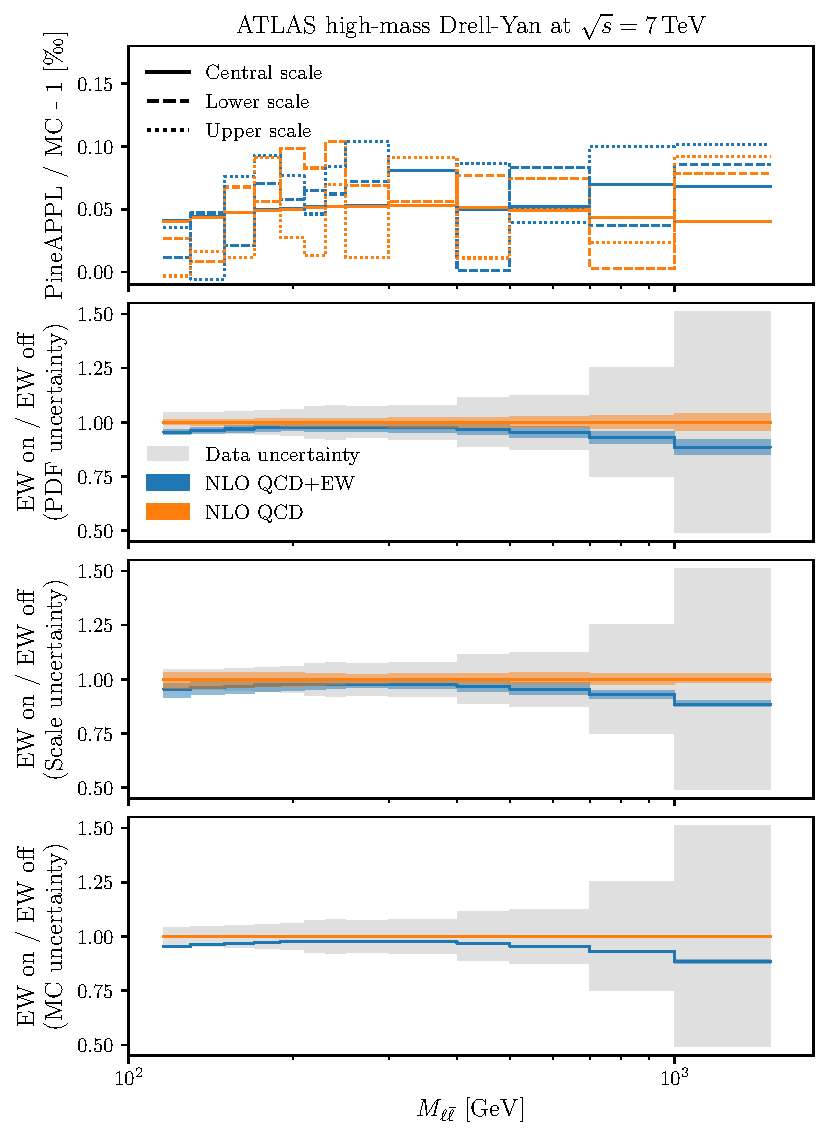
\includegraphics[width=0.5\textwidth]{figures/pineappl_ATLASZHIGHMASS49FB}
    \caption{Validation and test of the \textsc{PineAPPL} grid for the ATLAS
      high-mass Drell--Yan lepton pair measurement in the high-mass region at
      a centre-of-mass energy of \SI{7}{\tera\electronvolt}~\cite{Aad:2013iua}. The first panel
      displays the relative difference (in per mille) between the {\sc PineAPPL}
      and the MC results for the central, upper and lower scale choices,
      for theories accurate to both NLO QCD and NLO QCD+EW. The second, third
      and fourth panels present the theoretical predictions, accurate to either
      NLO QCD or NLO QCD+EW, always normalised to the former; on top of the
      theoretical predictions, the PDF uncertainty, the scale uncertainty and
      the Monte Carlo uncertainty are displayed in turn. The relative
      uncertainty of the experimental data is also shown for comparison.}
    \label{fig:atlaszhighmass49fb}
\end{figure}
%-------------------------------------------------------------------------------

The measurement is mainly driven by $\mathrm{q}\bar{\mathrm{q}}$ scattering: specifically, the
leading (next-to-leading) contribution comes from a $\mathrm{u}\bar{\mathrm{u}}$ ($\mathrm{d}\bar{\mathrm{d}}$)
parton luminosity, which accounts for about \SI{55}{\percent} (\SI{49}{\percent}) of the cross section
for the lowest invariant mass bins, and \SI{68}{\percent} (\SI{22}{\percent}) for the largest invariant
mass bins. The PI contribution raises from about \SI{1.3}{\percent} in the lowest bin to
about \SI{3.6}{\percent} in the highest bin. Overall, the EW corrections range between \SI{5}{\percent}
around $M_{\ell\bar\ell}\sim \SI{150}{\giga\electronvolt}$, \SIrange{2}{3}{\percent} for intermediate invariant mass
values, $\SI{150}{\giga\electronvolt}\lesssim M_{\ell\bar\ell}\lesssim \SI{700}{\giga\electronvolt}$, and
\SIrange{15}{20}{\percent} for the largest invariant mass bin, $M_{\ell\bar\ell}>\SI{1000}{\giga\electronvolt}$,
see figure~\ref{fig:atlaszhighmass49fb}. For this reason, the data points with
$M_{\ell\bar\ell}>\SI{210}{\giga\electronvolt}$ were not included in the NNPDF3.1
analysis~\cite{Ball:2017nwa}.

The NLO QCD+EW corrections always lead to a reduction of the cross section in
comparison to the NLO QCD prediction. The size of this shift is comparable to
the data uncertainty at small values of $M_{\ell\bar\ell}$, and rapidly becomes
negligible with respect to it as the value of the invariant mass increases
and the data uncertainty blows up. This fact suggests a couple of observations
in light of the inclusion of EW corrections in a fit of PDFs. First, the
description of the more precise bins in the low invariant mass range is likely
to change, and will possibly become more accurate should the inclusion of EW
corrections improve the data/theory agreement. Second, the kinematic cut that
excludes any data point at large $M_{\ell\bar\ell}$ can be safely removed: any
shift in the predictions induced by the more accurate NLO QCD+EW theory is
likely to be easily accommodated by the large data uncertainty.

In comparison to the PDF uncertainty, the size of the EW corrections is
always larger, especially at the boundaries of the distribution. This fact
suggests that, once included in a global fit, EW corrections could recast the
relative weight of each data set included in the fit, and possibly lead to
an improvement in their overall description. In comparison to the scale
uncertainty, the size of the EW correction is similar, except for the four bins
at the largest invariant mass, where the latter is significantly larger than
the former. The size of the scale variation is the same for the QCD and the
QCD+EW theories. These facts suggest that the NNLO QCD correction is comparable
to the NLO QCD+EW correction, except at very large values of the invariant mass,
where the EW correction still dominates. This result stresses the need to
include the EW corrections in order to obtain an accurate description of the
large invariant mass bins. Finally, the Monte Carlo statistical
uncertainty remains negligible in comparison to the data, PDF and scale
uncertainties, and to the size of the EW correction. Our conclusions are
therefore not affected by a poor simulation of the underlying events.

We then turn our attention to the double-differential measurement performed by
the CMS experiment at \SI{7}{\tera\electronvolt}. For illustrative purposes, we report only four out
of the six invariant mass bins, respectively below the Z-boson mass peak,
$\SI{45}{\giga\electronvolt}<M_{\ell\bar\ell}<\SI{60}{\giga\electronvolt}$, on the Z-boson mass peak,
$\SI{60}{\giga\electronvolt}<M_{\ell\bar\ell}<\SI{120}{\giga\electronvolt}$, above the mass peak,
$\SI{120}{\giga\electronvolt}<M_{\ell\bar\ell}<\SI{200}{\giga\electronvolt}$, and at very high invariant masses,
$\SI{200}{\giga\electronvolt}<M_{\ell\bar\ell}<\SI{1500}{\giga\electronvolt}$, see figure~\ref{fig:cmsdy2d11_bins3456}.
Analogous plots for the remaining low invariant mass bins are collected in
appendix~\ref{app:add_plots}. From figure~\ref{fig:cmsdy2d11_bins3456},
first of all we validate the \textsc{PineAPPL} result: its relative difference
with respect to the MC result is always below a fraction of per mille,
again irrespective of the accuracy of the theory, of the choice of scale, and
of the kinematic bin considered. 

%-------------------------------------------------------------------------------
\begin{figure}[!p]
    \centering
    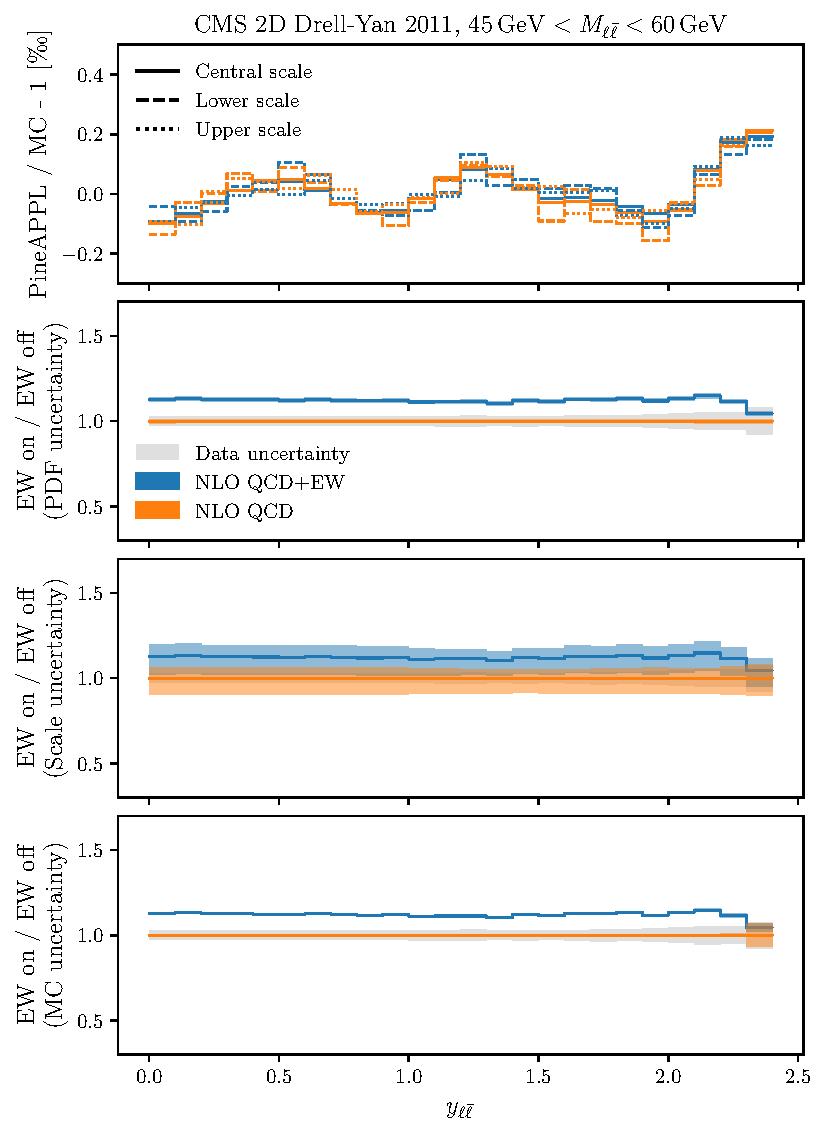
\includegraphics[width=0.5\textwidth]{figures/pineappl_CMSDY2D11_bin3}%
    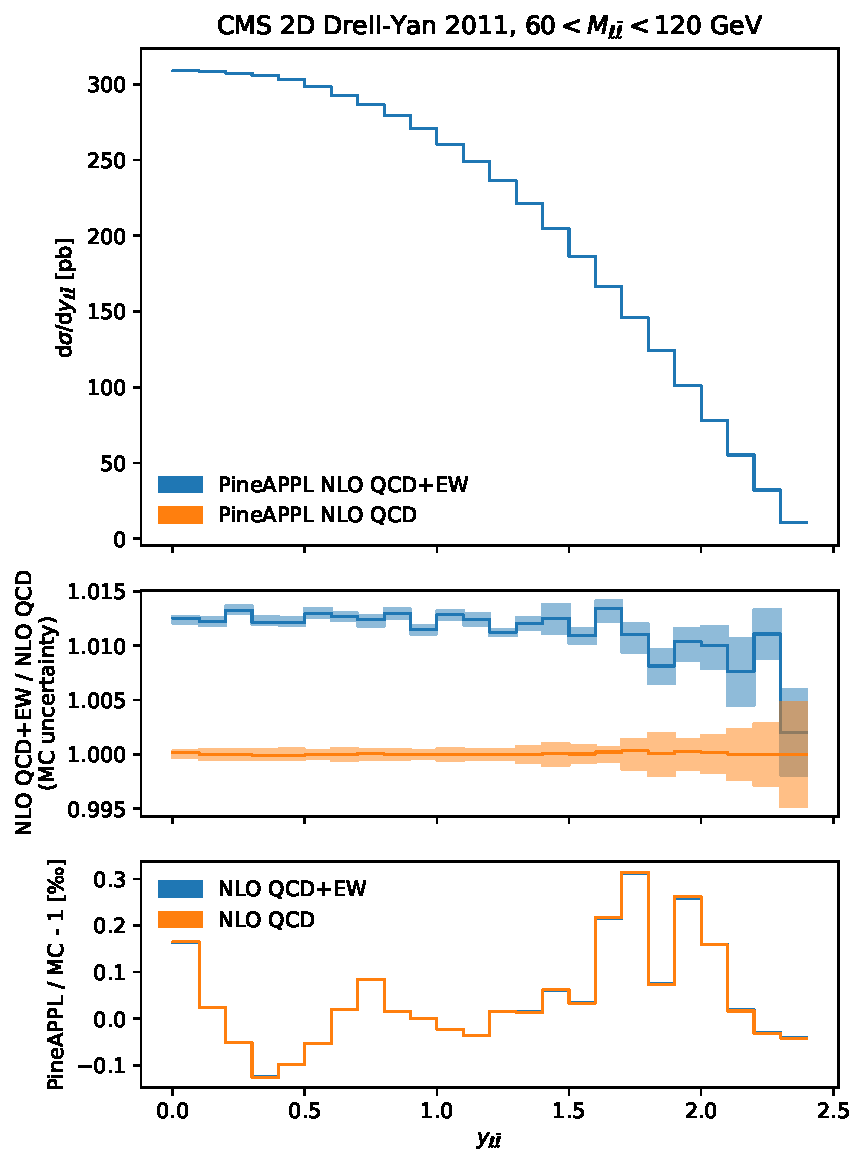
\includegraphics[width=0.5\textwidth]{figures/pineappl_CMSDY2D11_bin4}\\
    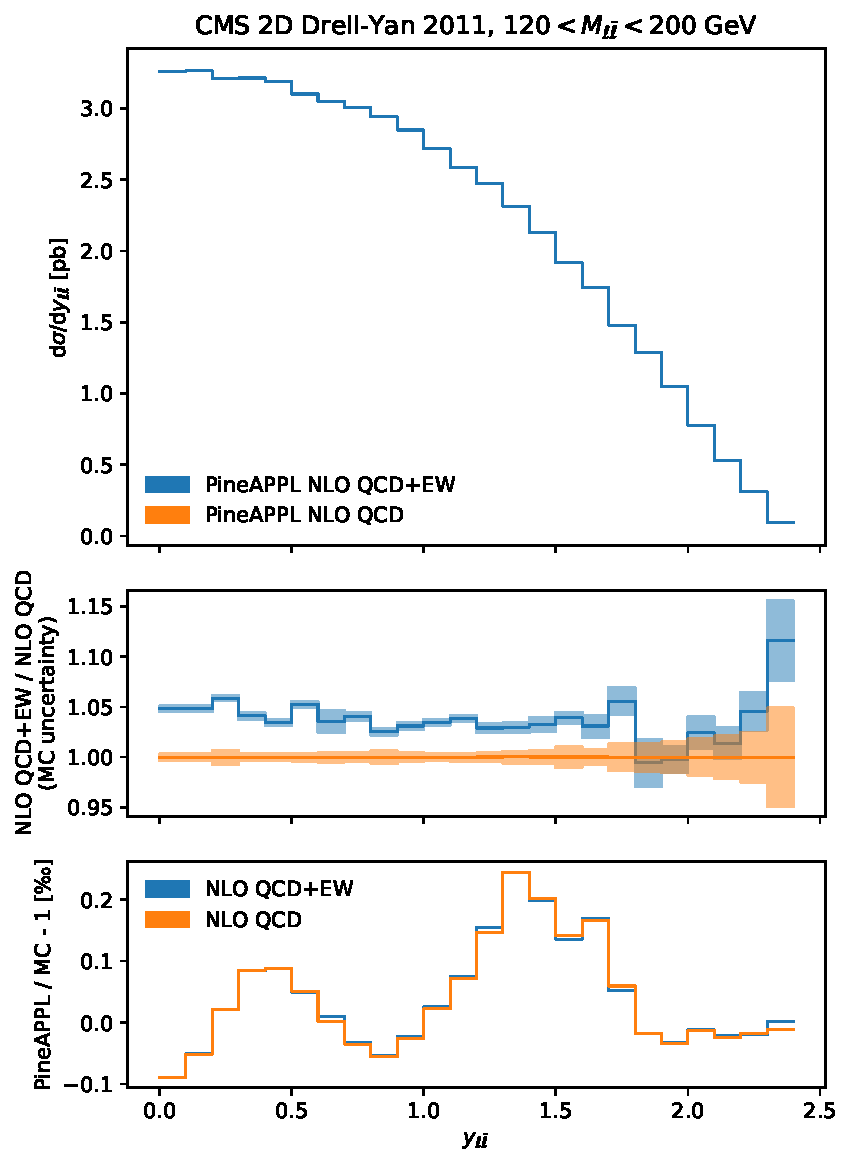
\includegraphics[width=0.5\textwidth]{figures/pineappl_CMSDY2D11_bin5}%
    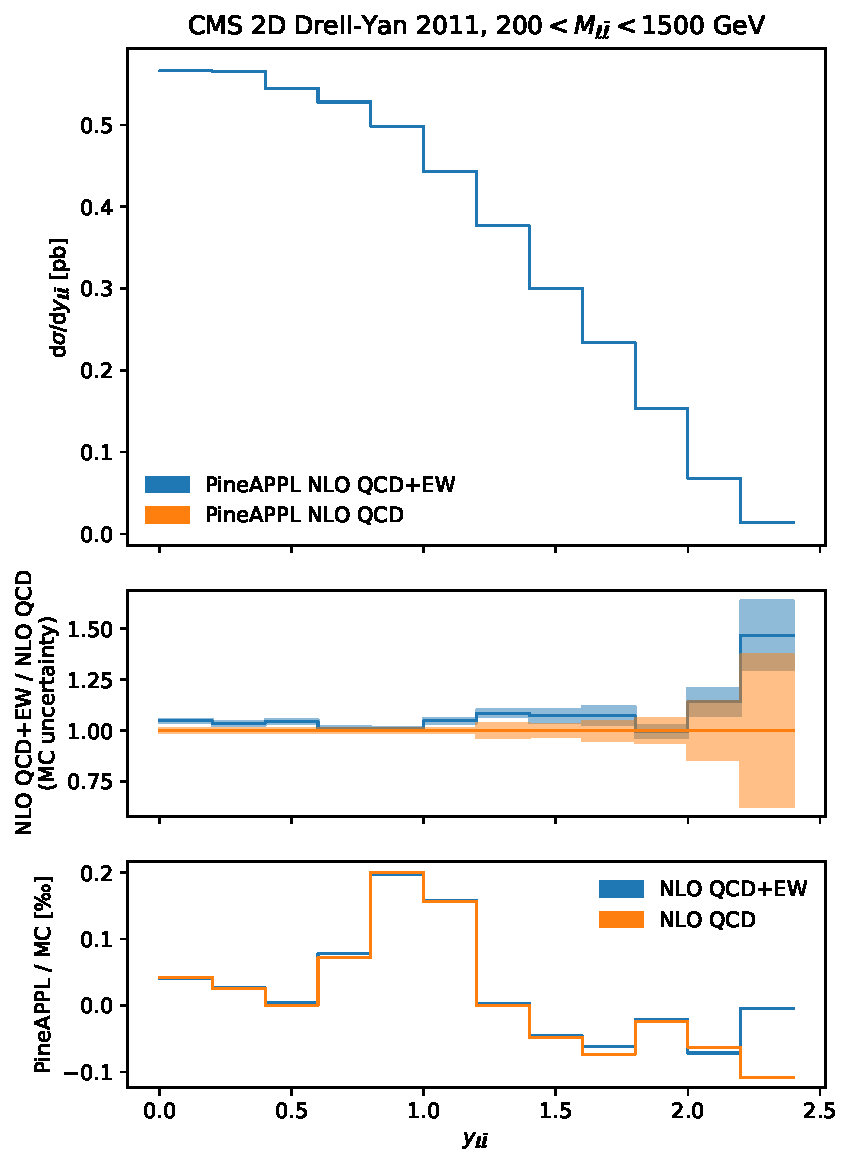
\includegraphics[width=0.5\textwidth]{figures/pineappl_CMSDY2D11_bin6}\\
    \caption{Same as figure~\ref{fig:atlaszhighmass49fb}, but for the CMS
      double-differential Drell--Yan lepton pair measurement at a
      centre-of-mass energy of \SI{7}{\tera\electronvolt}~\cite{Chatrchyan:2013tia}. Displayed are
      only two of the six invariant mass bins available, respectively below the
      Z-boson mass peak, $\SI{45}{\giga\electronvolt}<M_{\ell\bar\ell}<\SI{60}{\giga\electronvolt}$, on the Z-boson mass
      peak, $\SI{60}{\giga\electronvolt}<M_{\ell\bar\ell}<\SI{120}{\giga\electronvolt}$, above the mass peak,
      $\SI{120}{\giga\electronvolt}<M_{\ell\bar\ell}<\SI{200}{\giga\electronvolt}$, and at very high invariant masses,
      $\SI{200}{\giga\electronvolt}<M_{\ell\bar\ell}<\SI{1500}{\giga\electronvolt}$.}
    \label{fig:cmsdy2d11_bins3456}
\end{figure}
%-------------------------------------------------------------------------------

As in the case of the ATLAS high-mass Drell--Yan measurement, the CMS
measurement is also dominated by $\mathrm{q}\bar{\mathrm{q}}$ scattering. The leading
(next-to-leading) contribution to the $\SI{45}{\giga\electronvolt}<M_{\ell\bar\ell}<\SI{60}{\giga\electronvolt}$ invariant
mass bin comes from
the $\mathrm{u}\bar{\mathrm{u}}$ ($\mathrm{d}\bar{\mathrm{d}}$) parton luminosity, which accounts for about \SI{70}{\percent}
(\SI{22}{\percent}) of the double differential cross section, with small fluctuations across
the rapidity range. The PI contribution decreases from about \SI{4}{\percent} at zero
rapidity to \SI{1.5}{\percent} in the largest rapidity bin. The situation is slightly
different in the $\SI{60}{\giga\electronvolt}<M_{\ell\bar\ell}<\SI{120}{\giga\electronvolt}$ invariant mass bin, where the
leading (next-to-leading) contribution comes instead from the $\mathrm{d}\bar{\mathrm{d}}$
($\mathrm{u}\bar{\mathrm{u}}$) parton luminosity, which accounts for about \SI{60}{\percent} (\SI{44}{\percent}) of the
double differential cross section at small rapidities, and for about \SI{56}{\percent} (\SI{50}{\percent})
at large rapidities. In the remaining two invariant mass bins, the leading
(next-to-leading) contribution comes again from the $\mathrm{u}\bar{\mathrm{u}}$ ($\mathrm{d}\bar{\mathrm{d}}$)
parton luminosity, which accounts for about \SIrange{69}{95}{\percent} (\SIrange{38}{30}{\percent}) and
\SIrange{57}{70}{\percent} (\SIrange{48}{34}{\percent}) of the cross section, respectively for
$\SI{120}{\giga\electronvolt}<M_{\ell\bar\ell}<\SI{200}{\giga\electronvolt}$ and $\SI{200}{\giga\electronvolt}<M_{\ell\bar\ell}<\SI{1500}{\giga\electronvolt}$ in the
corresponding rapidity intervals; PI contributions range between \SIrange{7.3}{1.2}{\percent}
and \SIrange{3.7}{0.6}{\percent} in the two invariant mass bins, respectively, for increasing
rapidity.

The way in which NLO QCD+EW corrections affect the theoretical prediction for
the double differential cross section (with respect to its counterpart accurate
to NLO QCD) depends on the invariant mass bin. In the
$\SI{45}{\giga\electronvolt}<M_{\ell\bar\ell}<\SI{60}{\giga\electronvolt}$ region, they enhance the value of the cross
section by about \SI{11}{\percent} across all the rapidity range; in the
$\SI{60}{\giga\electronvolt}<M_{\ell\bar\ell}<\SI{120}{\giga\electronvolt}$ region, they suppress the value of the cross
section by about \SI{2}{\percent}, again across all the rapidity range; in the
$\SI{120}{\giga\electronvolt}<M_{\ell\bar\ell}<\SI{200}{\giga\electronvolt}$ bin, the suppression is around \SIrange{4}{5}{\percent}; and in
the $\SI{200}{\giga\electronvolt}<M_{\ell\bar\ell}<\SI{1500}{\giga\electronvolt}$ bin, the suppression increases further to
about \SIrange{6}{7}{\percent} for rapidities $y_{\ell\bar\ell}<2.0$ and up to \SIrange{20}{40}{\percent} at forward
rapidities. For this reason, for instance, the data points with
$M_{\ell\bar\ell}>\SI{200}{\giga\electronvolt}$ and $y_{\ell\bar\ell}>2.2$ were not included in the
NNPDF3.1 analysis~\cite{Ball:2017nwa}.

In general, the size of the EW corrections is comparable to or slightly larger
than the data uncertainty, except for the invariant mass bin 
$\SI{45}{\giga\electronvolt}<M_{\ell\bar\ell}<\SI{60}{\giga\electronvolt}$, where the shift due to the EW correction
overshoots the data uncertainty by about a factor of ten, and at large
rapidities, where the shift due to the EW correction, although it can become
large, is always a fraction of the data uncertainty. As already observed in the
case of the ATLAS measurement, should EW corrections be included in a fit of
PDFs, the description of the precise bins in the low invariant mass range is
likely to benefit from the more accurate theory; furthermore, the kinematic cut
that excludes any data point at large invariant mass and/or rapidity can be
safely removed.

In comparison to the PDF uncertainty, the size of the EW corrections is always
larger. We therefore anticipate that, once included in a PDF fit, they would
recast the relative weight of each data set included in the fit, and possibly
lead to an improvement in their overall description. In comparison to the scale
uncertainty, the size of the EW correction is similar, except on the Z-boson
mass peak, $\SI{60}{\giga\electronvolt}<M_{\ell\bar\ell}<\SI{120}{\giga\electronvolt}$, where the scale uncertainty exceeds
the size of the EW correction by about a factor of five. These facts confirm,
as expected, that EW corrections are almost immaterial at the Z-boson mass
peak, but that NNLO QCD corrections are otherwise as relevant as NLO QCD+EW
corrections. Finally, the Monte Carlo statistical uncertainty remains negligible
in comparison to the data, PDF and scale uncertainties, and to the size of the
EW correction, except for a couple of bins at forward rapidity in the highest
invariant mass bins. Improving the Monte Carlo statistical precision will
require to generate an unrealistically large number of events; therefore, it
might be desirable to treat this uncertainty as an additional theoretical
uncertainty in the PDF fit~\cite{Ball:2018lag}.

\paragraph{Top-quark pair production.} We now consider the top-pair differential
distributions measured by the ATLAS and CMS experiments at
\SI{8}{\tera\electronvolt}. In figure~\ref{fig:atlastop} we report the
distributions differential in the transverse momentum of the top quark,
$p_\mathrm{T}^\mathrm{t}$, and in the invariant mass of the top-quark pair,
$m_{\mathrm{t}\bar{\mathrm{t}}}$. Analogous plots for the distributions differential
in the rapidity of either the top quark or the top-quark pair are collected in
appendix~\ref{app:add_plots}. From figure~\ref{fig:atlastop}, we immediately
validate the \textsc{PineAPPL} result: its relative difference with respect to
the MC result is at most as large as $0.4\tcperthousand$, irrespective of the
accuracy of the theory, of the choice of scale and of the distribution
considered.

%-------------------------------------------------------------------------------
\begin{figure}[!t]
    \centering
    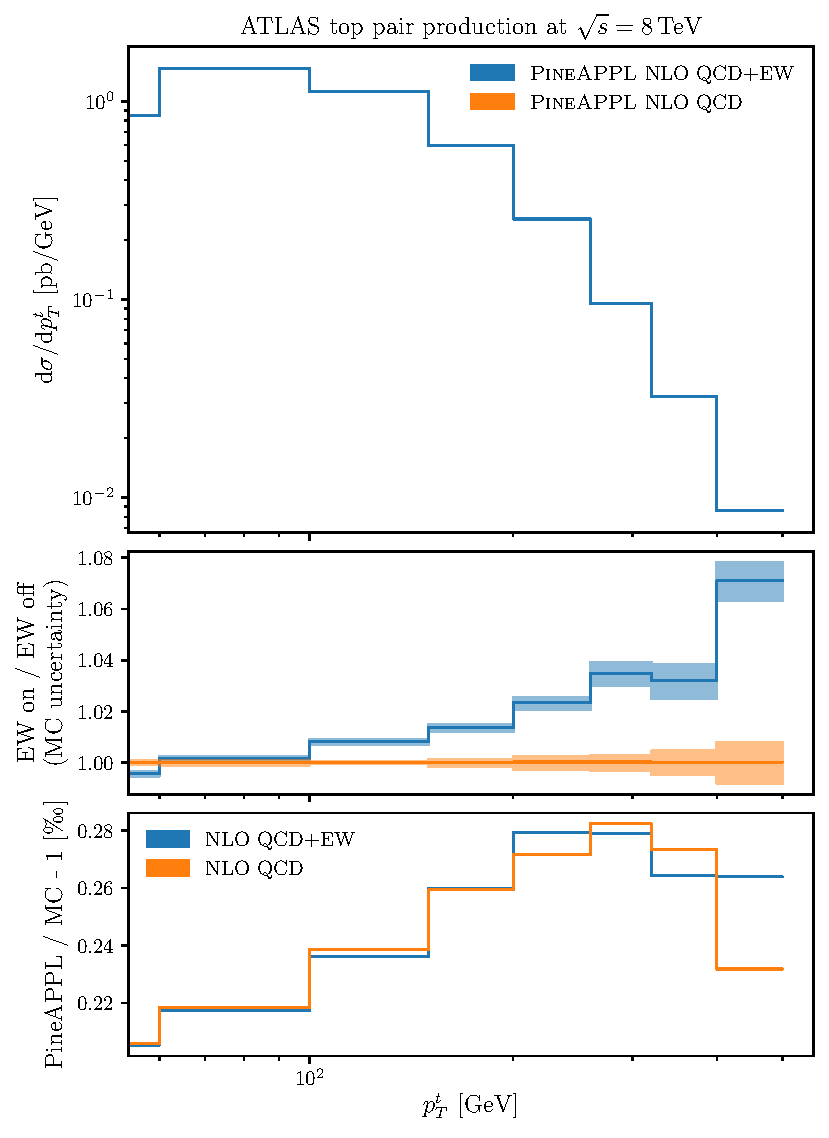
\includegraphics[width=0.5\textwidth]{figures/pineappl_ATLAS_TTB_DIFF_8TEV_LJ_TPT}%
    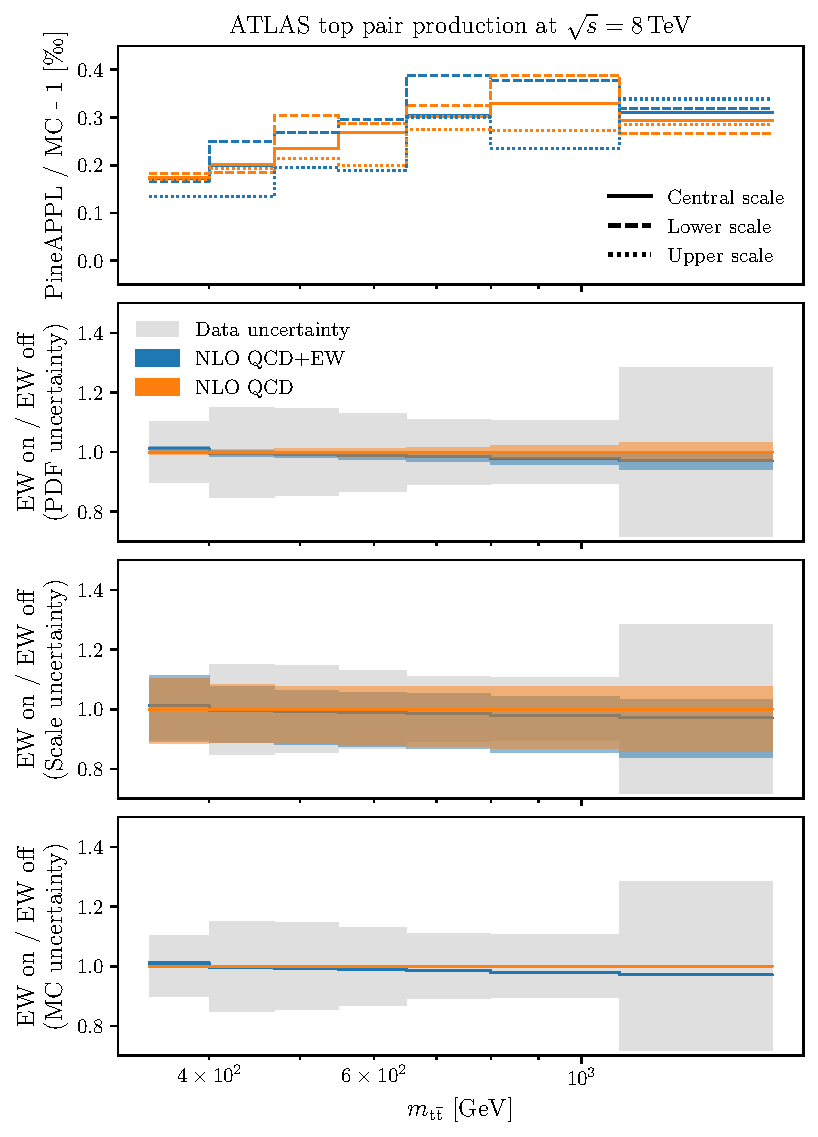
\includegraphics[width=0.5\textwidth]{figures/pineappl_ATLAS_TTB_DIFF_8TEV_LJ_TTM}
    \caption{Same as figure~\ref{fig:atlaszhighmass49fb}, but for the ATLAS
      differential top-quark pair measurement at a centre-of-mass energy of
      \SI{8}{\tera\electronvolt}~\cite{Aad:2015mbv}. Displayed are the distributions in the
      transverse momentum of the top quark $p_\mathrm{T}^\mathrm{t}$ (left), and in the invariant
      mass of the top-quark pair $m_{\mathrm{t}\bar{\mathrm{t}}}$ (right).}
    \label{fig:atlastop}
\end{figure}
%-------------------------------------------------------------------------------

The process receives its leading contribution from the $\mathrm{gg}$ channel,
which varies between 81\% and 61\% (76\% and 83\%) of the $p_\mathrm{T}^\mathrm{t}$
($m_{\mathrm{t}\bar{\mathrm{t}}}$) differential cross section as the value of the
transverse momentum of the top quark (the invariant mass of the top-quark pair)
increases in the bin range; $\mathrm{\gamma}\mathrm{g}$ scattering
correspondingly accounts for about 0.5\% -- 1\% (0.5\% -- 0.7\%) of the cross
section; the contribution from other PI parton luminosities is comparatively
negligible. Overall, the EW corrections suppress the $p_\mathrm{T}^\mathrm{t}$
($m_{\mathrm{t}\bar{\mathrm{t}}}$) distribution by about 0.2\% -- 3.5\%
(0.5\% -- 0.2\%) for increasing values of $p_\mathrm{T}^\mathrm{t}$
($m_{\mathrm{t}\bar{\mathrm{t}}}$), except in the first bin of the
$p_\mathrm{T}^\mathrm{t}$ distribution, where they enhance the cross section by
about 1\%. The size of these shifts, however, remains always significantly
smaller than the data uncertainty.\footnote{In
  figure~\ref{fig:atlastop} the data uncertainty corresponds to the ATLAS
  measurement~\cite{Aad:2015auj}. Similar considerations apply also for the CMS
  measurement~\cite{Khachatryan:2015oaa}.}
As a consequence, we anticipate that the more accurate NLO QCD+EW theory is
likely to be easily accommodated by the large data uncertainty, should the data
be fitted with the inclusion of EW corrections; PDFs will possibly not become
more precise.

The size of the EW correction is comparable to the size of the PDF uncertainty,
except at large values of transverse momentum or invariant mass, where the
former becomes larger than the latter. This fact suggests that, once included in
a global fit, EW corrections can improve the accuracy of the PDFs. In comparison
to the scale uncertainty, the size of the EW corrections remains negligible:
despite the fact that the choice of factorisation and renormalisation scales
have been devised to optimise the convergence of the perturbative expansion,
NNLO QCD corrections remain large, as expected in a process mostly initiated
by gluons. Their inclusion is therefore mandatory in a fit of PDFs. Finally,
the Monte Carlo statistical uncertainty remains negligible in comparison to the
data, PDF and scale uncertainties, and to the size of the EW correction. Our
conclusions are therefore not affected by Monte Carlo inefficiencies.

\paragraph{Z-boson production with non-zero transverse momentum.}

%-------------------------------------------------------------------------------
\begin{figure}[!t]
    \centering
    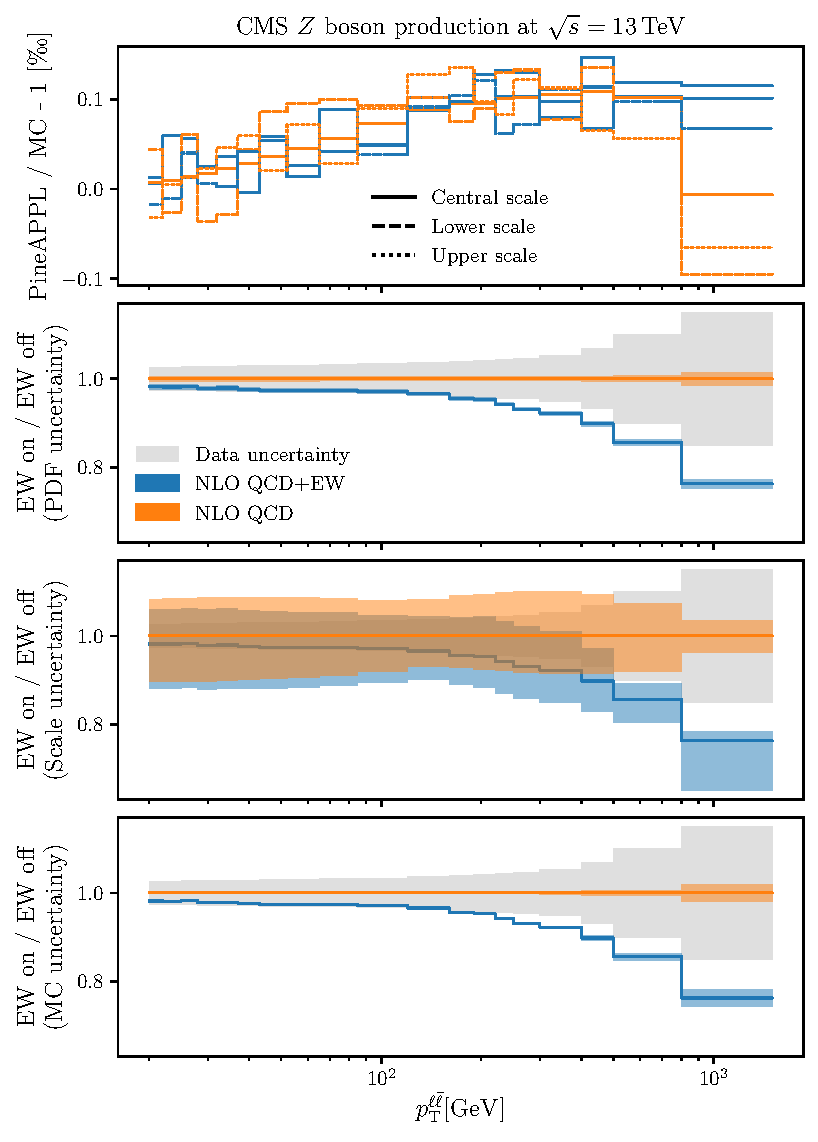
\includegraphics[width=0.5\textwidth]{figures/pineappl_CMS_Z_13_TEV}
    \caption{Same as figure~\ref{fig:atlaszhighmass49fb} but for the 
      CMS differential Z $p_\mathrm{T}$ measurement at a centre-of-mass energy of
      \SI{13}{\tera\electronvolt}~\cite{Sirunyan:2019bzr}.}
    \label{fig:cmsZ13TeV}
\end{figure}
%-------------------------------------------------------------------------------

\section{Subtraction of EW effects from data}
\label{sec:doublecounting}

The ability to include theoretical calculations of EW corrections in
PDF determinations, as has been mentioned in the introduction, is not enough to make a \emph{consistent} fit possible. Indeed, experimental data should
be provided in a format that allows PDF collaborations to easily employ them in these fits in a theoretically sound manner. Before concluding the paper,
we will provide some guidelines to facilitate a consistent presentation of experimental data to that end. We focus on the problem of data with (partially) subtracted EW effects, which, in PDF fits with theory predictions including them, leads to double counting of these EW effects.

\begin{figure}
    \centering
    \begin{overpic}[width=0.6\textwidth, trim=0.cm 11cm 0.cm 10cm, clip=True]{figures/dy-pi}
        \put (5, 33) {\large $\mathrm{q}$}
        \put (20, 37) {\large $\mathrm{q}$}
        \put (38, 5) {\large $\bar{\ell}$}
        \put (38, 31) {\large $\ell$}
        \put (11, 6) {\large $\gamma$}
        %
        \put (65, 9) {\large $\mathrm{q}$}
        \put (73, 30) {\large $\mathrm{q}$}
        \put (96, 25) {\large $\ell$}
        \put (96, 8) {\large $\bar{\ell}$}
        \put (55, 26) {\large $\gamma$}
    \end{overpic}
    \caption{\label{fig:dy-pi}
    Photon-induced (left) and quark-induced (right) contributions to the Drell-Yan process. In black, the LO process is shown.
    In red, the initial-state splitting leading to the real-emission $\mathrm{q} \gamma \to \ell \bar{\ell} \mathrm{q}$ is highlighted. Such a
    real emission enters in the NLO EW corrections.}
\end{figure}
An example is the subtraction of (irreducible) background processes which must not be considered as such. A very blatant case
is neutral-current Drell--Yan, where the signal process is the production of an opposite-sign lepton pair, which starts
at $\mathcal O(\alpha^2)$. Because this process is usually thought
as a quark-initiated $s$-channel mechanism ($\mathrm{q} \bar{\mathrm{q}} \to \gamma^*/\mathrm{Z} \to \ell \bar{\ell}$), in many analyses the photon-induced component,
$\gamma \gamma \to \ell \bar{\ell}$ in the $t$ channel, is considered to be a different process, and therefore as a background and subtracted.
The subtraction from the measured data is done by calculating the theoretical predictions of the double-photon initiated contribution, possibly including (ill-defined) higher-order
corrections. For example, in refs.~\cite{Aaboud:2017ffb,Aad:2016zzw} (a similar statement appears also in an older analysis~\cite{Aad:2013iua}), one reads:
\begin{quote}
The photon-induced process, $\gamma\gamma \to \ell \bar{\ell}$, is simulated at LO using Pythia 8
and the MRST2004qed PDF set~\cite{Martin:2004dh}. The expected yield for this process also accounts for 
NLO QED/EW corrections from references~\cite{Bardin:2012jk,Bondarenko:2013nu}, which decrease the yield by approximately \SI{30}{\percent}.
\end{quote}
Such a distinction, which is unphysical and incorrect in quantum mechanics, may be somehow justified at LO. Beyond this order, it is simply wrong.
Indeed, at $\mathcal O(\alpha^3)$, the reaction $\mathrm{q} \gamma \to \ell \bar{\ell} \mathrm{q}$ becomes possible, which
includes both kind of topologies discussed above, and needs both in order to yield an IR-finite result, see Fig.~\ref{fig:dy-pi} (as a consequence, one cannot speak of EW corrections to $\gamma \gamma \to \ell \bar{\ell}$). While it is common sense that the QCD counterpart of this subtraction should never 
be performed --- no one would
consider to \enquote{subtract} the gluon-initiated contribution to top-pair production in top analyses --- seemingly it is not so
when EW corrections are considered.

A second example is related to removing EW effects from data. These can be either the full EW corrections
or just a part of them. In either case, a comparison between these data and a NLO-EW accurate simulation aimed at the extraction of some parameter would be meaningless, as some effects included in the latter
have been removed from the former. The typical example relevant for LHC is the deconvolution of effects due to multiple-photon radiation
from light particles in the final state. This applies mostly
to processes such as neutral- or charge-current Drell--Yan, especially when electrons are considered. The problem lies in the fact that
 electrons, and to a lesser extent muons, tend to radiate photons, which are not accounted
for in QCD-only matrix-elements. Thus, leptons that are measured in the detector are less energetic, and this fact is compensated for
by inverting a photon shower. The resulting dataset is e.g.\ referred to as \emph{pre-FSR} with observables defined in terms of \emph{Born-level electrons} (see e.g.\ ref.~\cite{Aad:2015auj} for its definition).
These datasets are needed for and correctly used in QCD-only PDF determinations, since the EW corrections to some DY observables can be significant, and excluding them would therefore degrade the quality of the fit.
However, in fits including fixed-order EW corrections the problem with this definition is that the first photon emission is included exactly at the matrix-element level. The inclusion of
subsequent emission would require the matching with the QED shower, which is not yet available for general processes.

It is interesting
to note that one can tune the QED parton shower to mimic NLO EW effects for specific processes and observables, so that a prediction only accurate at NLO
QCD displays a remarkable agreement with another at NLO QCD+EW when the photonic shower is included (see for example the behaviour of predictions showered with
\textsc{Photos}~\cite{Barberio:1990ms,Barberio:1993qi,Golonka:2005pn} in ref.~\cite{CarloniCalame:2016ouw}). However, this kind of agreement
always comes \emph{a posteriori}, and cannot be ensured in general.
Furthermore, the deconvolution of QED effects in data introduces a dependence on the program (and possibly on 
the specific version) employed for the shower inversion. 
This fact is especially problematic if deconvolved datasets are the only ones which are published, since undoing the exact deconvolution can be very difficult, or practically impossible, as time passes. (TODO insert comment about LEP ISR and DIS EW effects removal).

A more physical definition of leptonic observables would be one making use of either bare leptons (the leptons as they emerge after FSR)
or of dressed leptons (leptons and photons are clustered together and their momenta are combined, in analogy with jets in QCD). The problem with the former is that 
electrons are never measured as bare particles, because of the finite resolution 
of the electromagnetic calorimeter. For what concerns muons, while in principle the concept of a bare muon is physical, it should be kept in
mind that modern, general-purpose codes employed to
compute EW corrections treat leptons as massless, to ensure numerical stability of the matrix elements. In this case, using bare leptons is not collinear safe.
Dressed leptons avoid all these shortcomings, with the further advantage of being
inclusive on the effect of extra collinear emissions. This fact encourages to explore the possibility of employing a dressed-lepton
definition, regardless of the leptonic flavour. It is reassuring to acknowledge that this practice is already being followed in experimental analyses:
indeed, to mention two examples of analyses discussed in this paper, in ref.~\cite{Aad:2015auj} data for dressed leptons are published, together with the Born-level
and bare ones, while refs.~\cite{Sirunyan:2019bzr} employs a dressed-lepton definition.

\section{Conclusions and Outlook}
\label{sec:conclusion}
The systematic inclusion of EW corrections in collider-physics simulations is crucial when high accuracy is required. Until
now, it was possible to include these effects only in one of the two ingredients of the physical cross section, namely
the short-distance (partonic) matrix element. For what concerns the second ingredient, PDFs, they were still extracted including
only QCD effects. In this paper, we amended to this situation, making it possible to include EW effects also in PDF fits.
We presented a new tool called \textsc{PineAPPL}, which stores perturbative calculations from an external Monte Carlo in a PDF-independent way using interpolation grids.
This offers the advantage of fast a-posteriori convolutions with PDFs, for example to study the uncertainties coming from different PDF sets and/or the strong coupling constant $\alphas$.
Another application that we focused on is PDF fitting, where the interpolation grids constitute the theoretical input.
We tested \textsc{PineAPPL} together with \textsc{mg5\_aMC@NLO} and found a precision of \numrange{e-4}{e-5} relative to the MC result, which is more than enough for the applications described before.
Although we used \textsc{mg5\_aMC@NLO}, we note that \textsc{PineAPPL} is not tied in any way to a specific MC and can be easily interfaced with any generator.

A distinguishing feature of \textsc{PineAPPL} is the support for arbitrary coupling orders not only in the strong, but also in the electroweak coupling.
This enables us to generate, for the first time, NLO EW and NLO combined QCD--EW interpolation grids.
Using \textsc{mg5\_aMC@NLO} we calculated and showcased the impact of these corrections for important PDF processes for specific analyses from ATLAS and CMS: Drell--Yan lepton-pair production, top-pair production, and Z-boson production with non-zero transverse momentum.

Finally, we discussed the issue of subtracting EW corrections in experimental data, which becomes an important consideration when combining the interpolation grids with the corresponding experimental data in a PDF fit including EW and combined QCD--EW corrections.

Having developed and thoroughly tested \textsc{PineAPPL}, all technical requirements are fulfilled for producing the first global PDF fit including EW and combined QCD--EW corrections.
This will have at least two advantages: in PDF fits phase-space regions are usually cut away if they exhibit large EW corrections; including them therefore increases the number of data points in a fit and therefore indirectly enlarges a PDF set's interpolation region.
Secondly, this makes it possible to use experimental data that are closer to the actual measurement, without the need to compensate for missing EW corrections.


\appendix

\acknowledgments

C.S. is supported by the European Research Council under the European Unions 
Horizon 2020 research and innovation Programme (grant agreement no.\ 740006).

\section{Installation and usage of \texorpdfstring{\textsc{PineAPPL}}{PineAPPL}}
\label{app:pineappl}

\subsection{Installation}
\label{app:installation}

\textsc{PineAPPL} currently consists of three parts: 1) the library itself, which is a dependency for the other parts, 2) the helper program \texttt{pineappl}, which allows one to read \textsc{PineAPPL} grids from the command line and make predictions with it, and finally 3) the C interface, which is intended to be used in Monte Carlo integrators to generate the grids.

\subsubsection*{Installation of Rust}

\lstset{
  basicstyle=\ttfamily\small,
  showstringspaces=false,
  commentstyle=\color{red},
  keywordstyle=\color{blue},
}

All parts are written in Rust: a Rust compiler and related tools are needed.
On operating systems with a \texttt{bash} shell (such as Linux or MacOS) the installation is as simple as
\begin{verbatim}
 $ curl --proto '=https' --tlsv1.2 -sSf https://sh.rustup.rs | sh
\end{verbatim}
which downloads the compiler \texttt{rustc}, the package manager \texttt{cargo}, and a few other helpful tools.
When the installation has completed make sure to read and follow the instructions printed on screen.
See also \url{https://www.rust-lang.org/tools/install} for more details and for installation instructions for other operating systems.

\subsubsection*{Installation of the command-line program \texorpdfstring{\texttt{pineappl}}{pineappl}}

The command-line program \texttt{pineappl} is compiled and installed using
\begin{verbatim}
 $ cargo install pineappl_cli
\end{verbatim}
This program also needs \texttt{LHAPDF} \cite{Buckley:2014ana} installed.
For usage instructions simply type \texttt{pineappl} in your shell and read the help message.

\subsubsection*{Installation of the C-language interface (optional)}

For the C interface you need to first install \texttt{cargo-c},
\begin{verbatim}
 $ cargo install cargo-c
\end{verbatim}
and then download the \textsc{PineAPPL} repository, compile and finally install into it into a directory \texttt{\$prefix} as follows:
\begin{verbatim}
 $ git clone https://github.com/N3PDF/pineappl/
 $ cd pineappl_capi/
 $ cargo cinstall --release --prefix=DIRECTORY
\end{verbatim}
The last line will install the C header \texttt{pineappl\_capi.h}, the library, and a pkg-config\footnote{A standard way on Linux to express how dependencies are compiled/linked against, see \url{https://www.freedesktop.org/wiki/Software/pkg-config/}} file (\texttt{pineappl\_capi.pc}) into the directory specified as \texttt{DIRECTORY}.
Make sure that the environment variables \texttt{PATH}, \texttt{LD\_LIBRARY\_PATH}, and \texttt{PKG\_CONFIG\_PATH} are properly set.
The latter is needed for \texttt{pkg-config -{}-cflags -{}-libs pineappl\_capi} to work, which prints the necessary compiler/linker flags.

After being installed, one can compile and link against the library.
See appendix~\ref{app:example-program} for an example.
Updated installation instructions are kept in the file \texttt{README.md} in \textsc{PineAPPL}'s repository at \url{https://github.com/N3PDF/pineappl/}.

\subsection{Example Monte Carlo program}
\label{app:example-program}

% TODO: link to documentation

\definecolor{mygreen}{rgb}{0,0.6,0}
\definecolor{mygray}{rgb}{0.5,0.5,0.5}
\definecolor{mymauve}{rgb}{0.58,0,0.82}

\lstset{
  belowcaptionskip=1\baselineskip,
  breaklines=true,
  frame=L,
  numbers=left,
  xleftmargin=\parindent,
  showstringspaces=false,
  basicstyle=\footnotesize\ttfamily,
  keywordstyle=\bfseries\color{green!40!black},
  commentstyle=\itshape\color{purple!40!black},
  identifierstyle=\color{blue},
  stringstyle=\color{orange},
}

The following listing shows how to setup \textsc{PineAPPL} using its C interface in a simple Monte Carlo integrator for calculating the double-photon contribution to Drell--Yan lepton-pair production at the LHC.
All \textsc{PineAPPL} functions have the prefix \texttt{pineappl\_}.
The full example can be found at \url{https://github.com/N3PDF/pineappl/tree/master/examples/capi-dy-aa}.

\begin{lstlisting}[language=C++,mathescape=true]
// create a new luminosity function for the $\gamma\gamma$ initial state
auto* lumi = pineappl_lumi_new();
int32_t pdg_ids[] = { 22, 22 };
double ckm_factors[] = { 1.0 };
pineappl_lumi_add(lumi, 1, pdg_ids, ckm_factors);

// only LO $\alpha_\mathrm{s}^0 \alpha^2 \log^0(\xi_\mathrm{R}) \log^0(\xi_\mathrm{F})$
uint32_t orders[] = { 0, 2, 0, 0 };

// we bin in rapidity from 0 to 2.4 in steps of 0.1
double bins[] = {
    0.1, 0.2, 0.3, 0.4, 0.5, 0.6, 0.7, 0.8, 0.9, 1.0, 1.1, 1.2,
    1.3, 1.4, 1.5, 1.6, 1.7, 1.8, 1.9, 2.0, 2.1, 2.2, 2.3, 2.4
};

// create the PineAPPL grid with default interpolation and binning parameters
auto* keyval = pineappl_keyval_new();
auto* grid = pineappl_grid_new(lumi, 1, orders, 24, bins, keyval);

// now we no longer need `keyval` and `lumi`
pineappl_keyval_delete(keyval);
pineappl_lumi_delete(lumi);

// fill the grid with phase-space points
fill_grid(grid, 10000000);

// perform a convolution of the grid with PDFs
auto* pdf = LHAPDF::mkPDF("NNPDF31_nlo_as_0118_luxqed", 0);
auto xfx = [](int32_t id, double x, double q2, void* pdf) {
    return static_cast <LHAPDF::PDF*> (pdf)->xfxQ2(id, x, q2);
};
auto alphas = [](double q2, void* pdf) {
    return static_cast <LHAPDF::PDF*> (pdf)->alphasQ2(q2);
};

std::vector<double> dxsec(24);
pineappl_grid_convolute(grid, xfx, xfx, alphas, pdf, nullptr,
    nullptr, 1.0, 1.0, dxsec.data());

// print the results
for (std::size_t i = 0; i != 24; ++i) {
    std::printf("%.1f %.1f %.3e\n", bins[i], bins[i + 1], dxsec[i]);
}

// write the grid to disk
pineappl_grid_write(grid, "DY-LO-AA.pineappl");

// destroy the object
pineappl_grid_delete(grid);
\end{lstlisting}

\subsection{Demonstration of \texorpdfstring{\texttt{pineappl}}{pineappl}}
\label{app:pineappl-demo}

The program \texttt{pineappl} can be used to perform quick convolutions and other calculations with existing grids on the command line.
If started without any arguments, it prints its help and lists all supported subcommands:
\begin{verbatim}
 $ pineappl
pineappl 0.2.0
Read, write, and query PineAPPL grids

USAGE:
    pineappl <SUBCOMMAND>

FLAGS:
    -h, --help       Prints help information
    -V, --version    Prints version information

SUBCOMMANDS:
    channels           Shows the contribution for each partonic channel
    convolute          Convolutes a PineAPPL grid with a PDF set
    diff               Compares the contents of two grids with each other
    info               Shows information about the grid
    luminosity         Shows the luminosity function
    merge              Merges one or more PineAPPL grids together
    orders             Shows the predictions for all bins for each order
                       separately
    pdf_uncertainty    Calculates PDF uncertainties
\end{verbatim}

\paragraph{Convolutions.}
The most important subcommand is \texttt{convolute}, which performs a convolution of a single grid with a single or multiple PDF sets.
As an example we show the grid produced for the ATLAS Drell--Yan high-mass lepton-pair production from section~\ref{subsec:numerical_results}, convoluted with \texttt{NNPDF31\_nlo\_as\_0118\_luxqed} as the main PDF set and with \texttt{CT18NLO} as a second PDF set.
\begin{verbatim}
 $ pineappl convolute ATLASZHIGHMASS49FB.pineappl \
 > NNPDF31_nlo_as_0118_luxqed CT18NLO
bin xmin xmax     diff        integ    neg unc pos unc       CT18NLO
---+----+----+------------+-----------+-------+-------+------------+------
  0  116  130 2.0630698e-1  2.888297e0  -2.08%   1.69% 2.0246802e-1 -1.86%
  1  130  150 9.1818985e-2  1.836379e0  -1.79%   1.86% 8.9766355e-2 -2.24%
  2  150  170 4.5306370e-2 9.061274e-1  -1.60%   1.98% 4.4115960e-2 -2.63%
  3  170  190 2.5894856e-2 5.178971e-1  -1.66%   2.06% 2.5138525e-2 -2.92%
  4  190  210 1.6075267e-2 3.215053e-1  -1.70%   2.10% 1.5566535e-2 -3.16%
  5  210  230 1.0526659e-2 2.105331e-1  -1.71%   2.12% 1.0173163e-2 -3.36%
  6  230  250 7.1928162e-3 1.438563e-1  -1.71%   2.13% 6.9403972e-3 -3.51%
  7  250  300 4.0776555e-3 2.038827e-1  -1.70%   2.44% 3.9255068e-3 -3.73%
  8  300  400 1.4775481e-3 1.477548e-1  -1.94%   2.87% 1.4182754e-3 -4.01%
  9  400  500 4.5473785e-4 4.547378e-2  -2.30%   3.19% 4.3525336e-4 -4.28%
 10  500  700 1.2164277e-4 2.432855e-2  -2.41%   3.12% 1.1612523e-4 -4.54%
 11  700 1000 1.9792340e-5 5.937701e-3  -2.05%   2.12% 1.8813113e-5 -4.95%
 12 1000 1500 2.0228761e-6 1.011438e-3  -1.29%   0.47% 1.9221978e-6 -4.98%
\end{verbatim}
The output shows all 13 bins with lower (\texttt{xmin}) and upper limit (\texttt{xmax}) of the invariant mass $M_{\ell \bar{\ell}}$ of the lepton pair, with the differential cross section $\mathrm{d} \sigma / \mathrm{d} M_{\ell \bar{\ell}}$ (\texttt{diff}), integrated cross section $(M_{\ell \bar{\ell}}^\mathrm{max} - M_{\ell \bar{\ell}}^\mathrm{min}) \mathrm{d} \sigma / \mathrm{d} M_{\ell \bar{\ell}}$ (\texttt{integ}), and the perturbative uncertainty estimated from a 7-point scale variation (envelope given by \texttt{neg unc} and \texttt{pos unc}).
The uncertainty estimation can alternatively use a 3- or a 9-point scale variation using the optional program switch \texttt{-{}-scales 3} or \texttt{-{}-scales 9}, respectively.
The (differential) results for the second PDF set (\texttt{CT18NLO}) is shown in absolute and relative (to first PDF set) numbers.

\paragraph{Perturbative orders.}
Often it is helpful to see the impact of the different perturbative orders to the cross section.
The subcommand \texttt{orders} shows this:
\begin{verbatim}
 $ pineappl orders ATLASZHIGHMASS49FB.pineappl \
 > NNPDF31_nlo_as_0118_luxqed
bin xmin xmax     diff     O(as^0 a^2) O(as^1 a^2) O(as^0 a^3)
---+----+----+------------+-----------+-----------+-----------
  0  116  130 2.0630698e-1     100.00%      15.97%      -5.26%
  1  130  150 9.1818985e-2     100.00%      18.07%      -4.29%
  2  150  170 4.5306370e-2     100.00%      19.66%      -3.64%
  3  170  190 2.5894856e-2     100.00%      20.69%      -3.21%
  4  190  210 1.6075267e-2     100.00%      21.26%      -2.91%
  5  210  230 1.0526659e-2     100.00%      21.48%      -2.85%
  6  230  250 7.1928162e-3     100.00%      21.60%      -2.62%
  7  250  300 4.0776555e-3     100.00%      21.36%      -2.75%
  8  300  400 1.4775481e-3     100.00%      20.32%      -3.11%
  9  400  500 4.5473785e-4     100.00%      17.83%      -3.65%
 10  500  700 1.2164277e-4     100.00%      14.04%      -4.68%
 11  700 1000 1.9792340e-5     100.00%       7.21%      -6.75%
 12 1000 1500 2.0228761e-6     100.00%      -3.05%      -9.99%
\end{verbatim}
The first four columns are the same as in \texttt{convolute}, and the remaining ones show all orders normalised to the sum of the leading orders, which in this case is only the $\mathcal{O} (\alpha^2)$.
Absolute numbers are shown if the switch \texttt{-{}-absolute} or \texttt{-a} is passed to the program.

\paragraph{Channels and Luminosity function.}
Sometimes it is useful to know which partons contribute the most and by how much.
This is what the subcommand \texttt{channels} shows:
\begin{verbatim}
 $ pineappl channels ATLASZHIGHMASS49FB.pineappl \
 > NNPDF31_nlo_as_0118_luxqed --limit 5
bin xmin xmax lumi  size
---+----+----+----+------+---+------+---+------+---+------+---+-----
  0  116  130  #15 27.42%  #0 27.42%  #5 24.52% #20 24.51% #30 1.30%
  1  130  150  #15 28.83%  #0 28.83%  #5 21.78% #20 21.78% #30 1.86%
  2  150  170  #15 29.87%  #0 29.82%  #5 19.63% #20 19.62% #30 2.32%
  3  170  190  #15 30.54%  #0 30.53% #20 18.17%  #5 18.13% #30 2.58%
  4  190  210   #0 31.06% #15 31.04%  #5 17.07% #20 17.04% #30 2.75%
  5  210  230   #0 31.46% #15 31.38% #20 16.27%  #5 16.24% #30 2.86%
  6  230  250   #0 31.73% #15 31.64% #20 15.66%  #5 15.62% #30 2.91%
  7  250  300   #0 32.07% #15 32.02%  #5 14.91% #20 14.86% #30 2.98%
  8  300  400   #0 32.62% #15 32.56%  #5 13.83% #20 13.81% #30 2.98%
  9  400  500  #15 33.14%  #0 33.12% #20 12.89%  #5 12.87% #30 2.93%
 10  500  700   #0 33.71% #15 33.31% #20 12.28%  #5 12.26% #30 2.93%
 11  700 1000  #15 34.08%  #0 33.71% #20 11.59%  #5 11.51% #30 3.06%
 12 1000 1500   #0 33.95% #15 33.88% #20 11.12%  #5 10.88% #30 3.56%
\end{verbatim}
The first three columns are known from \texttt{convolute}.
The next columns (the switch \texttt{-{}-limit 5} limits the output to five columns) show first the channel index and then the relative size of the corresponding contribution.
Since the contribution of a partonic channel can be negative, the columns are sorted ignoring the sign of the contribution.
The first line shows that for bin 0, i.e.\ for the range $\SI{116}{\giga\electronvolt} < M_{\ell \bar{\ell}} < \SI{130}{\giga\electronvolt}$, the cross section is dominated by partonic channel \texttt{\#15} (\SI{27.42}{\percent}), following by partonic channel \texttt{\#0}, then \texttt{\#5}, etc.
The meaning of the channel numbers is given by using the subcommand \texttt{luminosity} (only an excerpt is shown):
\begin{verbatim}
id    entry
--+------------+------------+------------
0  1 × ( 2, -2) 1 × ( 4, -4)
5  1 × ( 1, -1) 1 × ( 3, -3)
15 1 × (-4,  4) 1 × (-2,  2)
20 1 × (-3,  3) 1 × (-1,  1)
30 1 × (22, 22)
\end{verbatim}
This shows that channel \texttt{\#0} represents the up-type quark--anti-quark contributions (shown with PDG id 2 and 4 for up and charm quarks, which have the same matrix elements), channel \texttt{\#15} is the same channel with its initial states transposed, channels \texttt{\#5} and \texttt{\#20} are the down-type quark--anti-quark channels, and channel \texttt{\#30} is the photon--photon channel.
The size of the remaining channels is smaller than the photon--photon channel.
The factors \texttt{1} are not important here, but in general they can contain CKM values that, if kept in the squared matrix elements, would not allow for sharing a single matrix element for different quark flavours and therefore slow down the calculation. A complete list of the most important channels and of their
contibution to the cross section for all of the processes discussed in
section~\ref{sec:results} is collected in appendix~\ref{app:lumis}.

\subsection{Sample runcard for \texorpdfstring{\textsc{mg5\_aMC}}{mg5\_aMC}}
\label{app:sample-runcard}

The following run card was used to produce the results shown in section~\ref{subsec:numerical_results}.
The only difference with respect to a standard \textsc{mg5\_aMC} run is the switch \texttt{set iappl 1}, which enables to fill a \textsc{PineAPPL} grid.
For a complete set of runcards and patches see TODO.

\begin{verbatim}
set complex_mass_scheme True
import model loop_qcd_qed_sm_Gmu
define p = p b b~
define j = p
generate p p > e+ e- [QCD QED]
output @OUTPUT@
launch @OUTPUT@
fixed_order = ON
set mz @MZ@
set ymt @YMT@
set ebeam1 3500
set ebeam2 3500
set pdlabel lhapdf
set lhaid 324900
set fixed_ren_scale True
set fixed_fac_scale True
set mur_ref_fixed @MZ@
set muf_ref_fixed @MZ@
set reweight_scale True
set ptl = 25.0
set etal = 2.5
set mll = 116
#user_defined_cut set mmllmax = 1500.0
set req_acc_FO 0.0001
set iappl 1
done
quit
\end{verbatim}


\bibliographystyle{JHEP}
\bibliography{paper}

\end{document}
